\PassOptionsToPackage{subsection=false}{beamerouterthememiniframes}
\documentclass[9pt,compress,t]{beamer}
\usetheme[
	bullet=circle,
	alternativetitlepage=true,
	titleline=true,
	titlepagelogo=img/loghi_insieme,
]{mathlab}
\usepackage[utf8]{inputenc}
\usepackage[T1]{fontenc}
\usepackage[english]{babel}
\usepackage{amsmath}
\usepackage{amsthm}
\usepackage{amsfonts}
\usepackage{graphicx}
\usepackage{caption}
\usepackage{subcaption}
\usepackage{verbatim} % per comment
\usepackage{lmodern} % font più chiaro
\usepackage{ragged2e}
\usepackage{bm}
\usepackage{tikz}
\usepackage[thicklines]{cancel}
\usepackage{xcolor}
\usepackage{wasysym}
\usepackage{units}
\usepackage{tikzsymbols}
\usepackage{multimedia}
\usepackage{graphicx}
%\usepackage{media9}%
\newcommand\Ccancel[2][black]{\renewcommand\CancelColor{\color{#1}}\cancel{#2}}
\newcommand{\cfbox}[2]{%
    \colorlet{currentcolor}{.}%
    {\color{#1}%
    \fbox{\color{currentcolor}#2}}%
}

%% matlab 2 tikz
\usepackage{pgfplots}
\pgfplotsset{compat=newest}
%% the following commands are needed for some matlab2tikz features
\usetikzlibrary{plotmarks}
\usetikzlibrary{arrows.meta}
\usetikzlibrary{positioning,arrows}
\usepgfplotslibrary{patchplots}
\usepackage{grffile}
\usepackage{amsmath}
\usepackage{graphicx}
\DeclareMathOperator*{\arginf}{arg\,inf}
%% end matlab 2 tikz


\setbeamertemplate{navigation symbols}{}


\graphicspath{%
	{img/}%
}

%\title[Here you put a short title]{\LARGE\bf Here it goes a possibly longer title}
\title[Parallel POD]{\LARGE\bf A multiprocess and multithreaded strategy\\ for parallel proper orthogonal decomposition\\ in a reduced order modeling framework}
\author[F. Krötz]{\vspace{-1cm}\\\textbf{Florian Krötz}} 
\institute[SISSA mathLab]{%
\vspace{-3mm}\\%
MathLab, Mathematics Area, SISSA International School for Advanced Studies, Trieste, Italy\\ \vspace{3mm}
Ulm University, Ulm, Germany \\
}
\date{\vspace{-3mm}\\ 19.06.2020 \\
}
% Norma
\newcommand\norm[1]{\left\lVert#1\right\rVert}

\usepackage{algpseudocode}
\usepackage[Algorithm]{algorithm}


% Evidenziato
\newcommand{\TODO}[1]{{\color{red}#1}}
\newcommand{\highlight}[1]{\textbf{\color{bluemathlab}#1}}
\newcommand{\highlightB}[1]{\textbf{\color{black!15!orangemathlab}#1}}
\newcommand{\mathhighlight}[1]{\color{bluemathlab}#1}
\newcommand{\mathhighlightB}[1]{\color{black!15!orangemathlab}#1}

% Framebreaks: move continuation count from subtitle to title
\setbeamertemplate{frametitle continuation}[from second][]
\makeatletter 
\long\def\beamer@@frametitle[#1]#2{% 
  \beamer@ifempty{#2}{}{% 
    \gdef\insertframetitle{#2\ifnum\beamer@autobreakcount>1\relax{}\space(\insertcontinuationcountroman)\fi}% 
  \gdef\beamer@frametitle{#2}% 
  \gdef\beamer@shortframetitle{#1}% 
}% 
}
\makeatother 

\setbeamercolor{blockcolor1}{fg=black,bg=bluemathlab!10}
\setbeamercolor{blockcolor2}{fg=black,bg=orangemathlab!10} 

\AtBeginSection[]
{{
%	\setbeamertemplate{footline}[decolines theme without pages]
	\addtocounter{framenumber}{0}
	%\begin{frame}
	%\frametitle{Table of contents}
	%\tableofcontents %[currentsection]
	%\end{frame}
}}

\begin{document}
% Titel page %%%%%%%%%%%%%%%%%%%%%%%%%%%%%%%%%%%%%%%%%%%%%%%%%%%%%%%%%%%%%%%%%%%
\begin{frame}[t,plain]
	\addtocounter{framenumber}{-1}
	\titlepage
\end{frame}
%%%%%%%%%%%%%%%%%%%%%%%%%%%%%%%%%%%%%%%%%%%%%%%%%%%%%%%%%%%%%%%%%%%%%%%%%%%%%%%%%
\begin{frame}{~}
	\Large{\highlightB{Agenda}}

	\vspace{0.2cm}
	\hspace{0.5cm}
	\begin{minipage}[t]{0.7\textwidth}
		\begin{enumerate}
			\item Reduced Basis Method
			\item Parallel POD algorithms
			\item Implementation and Benchmarks
			\item Integration in \texttt{EZyRB} with an example
		\end{enumerate}
		
	\end{minipage}	


	
	
\end{frame}

\begin{frame}{Motivation}
	\Large{\highlightB{Physical Problems}}
	\normalsize
	
	Complex phenomena described using \highlightB{parametrized} \highlight{Partial Differential Equations (PDE)}
	\begin{minipage}{\textwidth}
		\vspace{0.5cm}
		\centering
		\begin{minipage}{0.25\textwidth}
			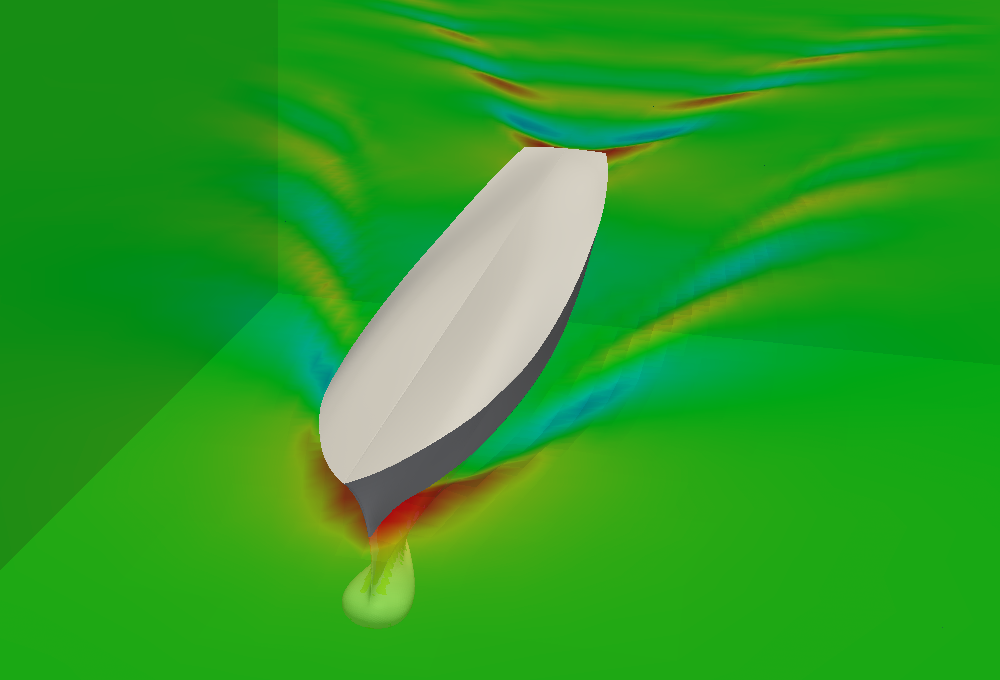
\includegraphics[width=\textwidth]{img/DTMB_orig.png}
			\centering
			Naval Engineering
		\end{minipage}\hspace{0.5cm}
		\begin{minipage}{0.25\textwidth}\hspace{1cm}
			
\includegraphics[width=\textwidth]{img/wing.jpg}
			\centering
			Aeronautics
		\end{minipage}\hspace{0.5cm}
		\begin{minipage}{0.25\textwidth}\hspace{1cm}
			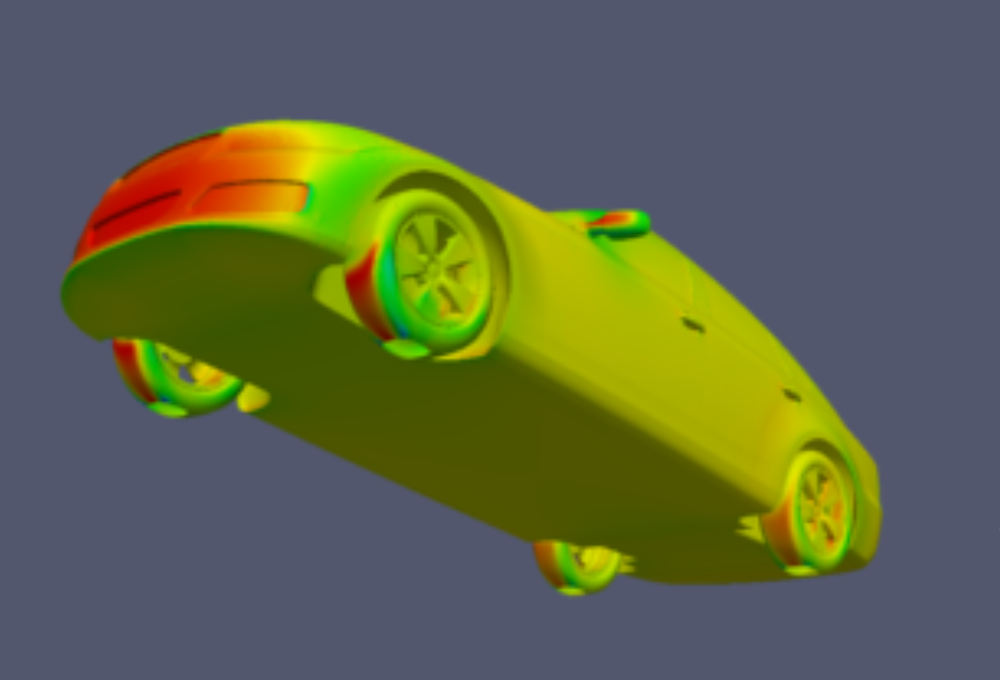
\includegraphics[width=\textwidth]{img/automotive.png}
			\centering
			Automotive 
		\end{minipage}
		\vspace{0.5cm}
	\end{minipage}

	Solving the PDEs using fine discretization like \highlight{Finite Element}, \highlight{Finite Volume}, ...

	\vspace{0.5cm}
	\highlight{Problem:} Many evaluations are expensive.
	\begin{itemize}
		\item \highlight{optimizing} the parameter (\highlight{multi query} application)
		\item \highlight{controlling} the parameter (\highlight{real time} application)
	\end{itemize}


	
\end{frame}



\chapter{Reduced Basis Method}
In this chapter, we give an overview on reduced basis (RB) methods. 
RB methods are used when we are interested in efficient solutions of the same parametric PDE for different parameters.
This can be the case in multi-queries applications like optimization or in real-time applications.

The workflow of RB methods can be divided into two phases, the offline-phase and the online-phase.

\begin{enumerate}
	\item In the offline-phase, we create a reduced model of the parametric PDE. 
	To create this reduced model we need so called truth solutions. These truth solutions are very good approximations of the exact solutions. We assume that the approximation is sufficiently good so that we can call them truth solutions.
	We create the truth solutions using a discretization technique. Finite Element (FEM) and Finite Volume (FV) are popular discretization techniques to compute the truth solutions.
	The most commonly used software packages by the scientific community are FEniCS \cite{LoggMardalEtAl2012} for FEM and OpenFOAM \cite{articleOpenFOAM} for FVM.
	These truth solutions have a high computational cost and they are usually calculated on a HPC supercomputer.	
	The truth solutions are used to create the reduced model. In this chapter we will describe how to create a reduced model using the proper orthogonal decomposition.

	\item In the online-phase, we solve the reduced model that we created in the offline-phase.
	This reduced problem requires much lower computational cost with respect to the previous phase. Solving the reduced problem can be done on less powerful hardware like a laptop, tablet, or smartphone.
\end{enumerate}

\begin{figure}[H]
	\centering
	\tikzset{
	main/.style={black, line width=0.4mm, opacity=1},
	second/.style={gray, opacity=5},
	arrow/.style={-latex, shorten >=1ex, shorten <=1ex, bend angle=45}
}
\begin{tikzpicture}
%% Global Matrix
\draw[main] (0,0) -- (2,0) -- (2,2)-- (0,2)-- (0,0);
\draw[main] (4,0) -- (6,0) -- (6,2)-- (4,2)-- (4,0);
\draw[main] (8,0) -- (10,0) -- (10,2)-- (8,2)-- (8,0);


\draw [arrow]  (2,1) to (4,1);
\draw [arrow]  (6,1) to (8,1);


\draw (1,1) node {$u(\mu)$};
\draw (5,1) node {$u^\mathcal{ N }(\mu)$};
\draw (9,1) node {$u_N(\mu)$};

\draw (3,1.5) node {FEM};
\draw (3,.5) node {FV};

\draw (7,1.5) node {RB};
\draw (7,.5) node {POD};

\draw (1,-.5) node {Hilbert space $\mathbb{X}$};
\draw (5,-.5) node {Truth space $\mathbb{X}^\mathcal{ N }$};
\draw (5,-1) node {offline-phase};
\draw (9,-.5) node {RB space $\mathbb{X}_N$};
\draw (9,-1) node {online-phase};


\end{tikzpicture}
	\caption[RB process]{Sketch of the RB workflow. Starting from the exact solution of the PDE $u(\mu)$.
		Then the offline-phase, where we are creating snapshot solution $u^\mathcal{ N }(\mu)$ in the truth space $\mathbb{X}^\mathcal{ N }$ using FEM or FV.
		And finally, in the online-phase where we are computing reduced solutions $u_N(\mu)$ in the RB space $\mathbb{X}_N$.}
	\label{fig:scetch}
\end{figure}

Before we start, a view remarks to the notation.
Everything associated with the exact solution has no indices.
Everything associated with the truth space has a superscripted calligraphic $\mathcal{ N }$ $\left(\cdot^\mathcal{ N }\right)$.
Everything associated with the RB space has a subscripted normal $N \left(\cdot_N\right)$.

We start with the weak formulation of a parametric PDE
\begin{align}
\text{find }u(\mu) \in \mathbb{X} :\quad a(u(\mu),v;\mu) = f(v;\mu) \quad \forall v \in \mathbb{X}.
\label{eq:weakform}
\end{align}

Where$\mathbb{X}$ is a Hilbert space in which we search for the solution,
$\mu \in \mathbb{R}^n$ is the parameter vector containing all the parameters that describe our parametrized PDE,
$a(\cdot,\cdot,\mu)$ is a parametric bilinear form containing the equation describing the physics,
$f(\cdot,\mu)$ is a parametric linear form containing the source term on the right-hand side and
$u(\mu)\in \mathbb{X}$ is the exact solution depending on $\mu$.

In a weak formulation, an equation is no longer required to be well defined and has instead weak solutions only with respect to certain "test functions". This is equivalent to formulating the problem to require a solution in the sense of a distribution.
In Section \ref{sec:HeatConduction} we make an example of the weak formulation for the heat equation.

The exact solution is not available in most cases, so first we need to approximate the solution as good as possible.
Because the Hilbert spaces are usually $ \infty $-dimensional, we need a sufficient fine discretization.
FEM and FV are popular discretization techniques to compute the solutions.
We call solutions, which are computed by these methods truth solutions.

These methods discretise  the  $ \infty $-dimensional space by choosing a finite number of basis functions $\{ \varphi_i^\mathcal{ N } \}_{i=1}^{\mathcal{ N }} \in \mathbb{X}$.
The basis functions $\varphi_i^\mathcal{ N }$ span the truth space
$\mathbb{X}^\mathcal{ N } = \text{span} \{ \varphi_1^\mathcal{ N }, ..., \varphi_\mathcal{N}^\mathcal{N}  \} \subset{X} $.
The choice of these basis functions depends on the discretization technique. 
The truth solutions are denoted with  $u^\mathcal{N}(\mu)$ where $\mathcal{N}$ stands for the degrees of freedom of the high fidelity solution.
The truth solution can be represented as a linear combination of basis functions
\begin{align}
\label{eq:truthSolution}
u^\mathcal{ N } (\mu) = \sum_{i=1}^\mathcal{ N } u_i^\mathcal{ N } (\mu) \cdot \varphi_i^\mathcal{ N },
\end{align}
where $ u_i^\mathcal{ N } (\mu)$ are coefficients that scale the basis functions in the linear combination.
Using the discretization, the truth problem can now be written as
\begin{align}
\label{eq:truthProblem}
\text{find }u^\mathcal{N}(\mu) \in \mathbb{X}^\mathcal{N} :\quad a(u^\mathcal{N}(\mu),v;\mu) = f(v;\mu) \quad \forall v \in \mathbb{X}^\mathcal{N}.
\end{align}


Using the discrete basis functions, the truth problem (\ref{eq:truthProblem}) leads to the discrete system 
\begin{align*}
\underline{A}^\mathcal{ N } (\mu) \underline{u}^\mathcal{ N } (\mu) = 
\underline{f}^\mathcal{ N }(\mu),
\end{align*}
with:
\begin{itemize}
	\item The stiffness matrix $\mathbf{A}^\mathcal{ N } (\mu) = [a(\varphi_i,\varphi_j,\mu)]_{i=1,...,\mathcal{N}}$ 
	\item The right hand side vector $\underline{f}^\mathcal{ N } (\mu) = [f(\varphi_j,\mu)]_{j=1,...,\mathcal{N}}$
	\item The solution vector $\underline{u}^\mathcal{ N } (\mu) = [u_i^\mathcal{ N }(\mu)]_{i=1,...,\mathcal{N}}$ containing  the coefficients $u_i^\mathcal{ N } (\mu)$. 
\end{itemize}

We define the discrete solution manifold
\begin{align*}
\mathbb{M^\mathcal{N}} = \{u^\mathcal{N}(\mu),\quad \mu \in \mathbb{P}\}.
\end{align*}
as the set of all truth solution varying the parameter.

In many cases it is too expensive to compute a truth solution for all parameters we are interested in.
The aim of RB methods is to approximate the solution manifold as good as possible but also efficiently.

The idea is to provide a projection to the manifold on low dimensional space using a small number of basis functions $\{\xi_i\}_{i=1}^{N}$.

A small number means that the number of basis functions is a lot smaller than the degrees of freedom of the high fidelity solution $N \ll \mathcal{ N }$.
The basis function spans the RB space $ \mathbb{X}_N = \text{span}(\xi_1, ...,\xi_N )\subset \mathbb{X}^\mathcal{ N } $.
Compared to (\ref{eq:truthSolution}) for the reduced solution, we want to use $N$ basis functions from the reduced basis instead of $\mathcal{ N }$ basis functions from the truth basis.
The reduced solutions are defined as a linear combination of reduced basis functions
\begin{align*}
u_N(\mu) = \sum_{i=1}^{N} u_{N,i}(\mu) \xi_i,
\end{align*}
where $ u_{N,i}(\mu)$ are the coefficients of the reduced system.

The reduced basis functions are build as a linear combination of truth basis functions
\begin{align}
\label{eq:basisfun}
\xi_i  = \sum_{k=1}^{\mathcal{ N }} b_{k,i} \varphi_k^\mathcal{ N },
\end{align}
with the coefficients  $b_{k,i}$. These coefficients are stored in the matrix $B \in \mathbb{R}^{\mathcal{ N } \times N}$. The $i$-th column of $B$ contains the coefficients for the $i$-th basis function $\xi_i$ \cite[Section 3.1]{HRSbook}.
A way to compute this basis, respectively the coefficients $b_{k,i}$, is the proper orthogonal decomposition (POD).
The POD will be described in detail in Section \ref{sec:POD}. 

Using the reduced basis functions, we can create the reduced system
\begin{align*}
\mathbf{A}_N (\mu) \underline{u}_N (\mu) = \underline{f}_N(\mu)
\end{align*}
with:
\begin{itemize}
	\item The reduced stiffness matrix $\mathbf{A}_N (\mu) = [a( \xi_i , \xi_j  ; \mu )]_{i,j=1,...,N}$
	\item The reduced right hand side vector $\underline{f}_N (\mu) = [f(\xi_j ; \mu)]_{j=1,...,N}$
	\item The solution vector $\underline{u}_N (\mu) = [ u_{N,i}(\mu) ]_{i=1,...,N}$ containing the coefficients $u_{N,i}(\mu)$
\end{itemize}
To compute the reduced stiffness matrix $\mathbf{A}_N (\mu)$ we insert the reduced basis functions into the bilinear form $a( \xi_i , \xi_j,  \mu )$.  
Since it is a bilinear form, we are able to write it as
\begin{align*}
a( \xi_i , \xi_j,  \mu ) =
\sum_{k=1}^{\mathcal{ N }} \sum_{l=1}^{\mathcal{ N }} b_{i,k} b_{j,l} a( \varphi_i , \varphi_j ;  \mu ).
\end{align*}
Computing this for every given $\mu$ would be a very high computational effort.
We assume the bilinear form $a(\cdot, \cdot, \mu)$ is affine in the parameter. Which means we can decompose it in functions $\theta_a^q(\mu)$ containing the parameter $\mu$ and bilinear forms $a^q( \varphi_i , \varphi_j )$ independent from the parameter.
We call this the affine decomposition 
\begin{align}
\label{eq:afdecomp}
a( \xi_i , \xi_j,  \mu ) =
\sum_{q=1}^{Q_a} \theta_a^q(\mu) \sum_{k,l=1}^{\mathcal{ N }} b_{i,k} b_{j,l} a^q( \varphi_i , \varphi_j ).
\end{align}
An example of such an affine decomposition is done in Section \ref{sec:HeatConduction}.
The last sum in (\ref{eq:afdecomp}) is independent from $\mu$ and can be computed in the offline phase. It can be written in matrix form
\begin{align*}
\mathbf{A}_N^q  = \mathbf{B}^T \mathbf{A}^{\mathcal{ N },q} \mathbf{B},
\end{align*}
where the matrices $\mathbf{A}^{\mathcal{ N },q}$ are the parameter independent parts of the truth system. With this operation we project the coefficients of the truth system into the reduced space.  
The same is done for the right hand side part $\underline{f}_N^q = \mathbf{B}^T  \underline{f}^{\mathcal{ N },q}$.


$  \mathbf{A}_N (\mu) $ and $ \underline{f}_N (\mu) $ can be build efficiently in the online phase
\begin{align*}
\mathbf{A}_N (\mu) = \sum_{q=1}^{Q_a} \theta_a^q(\mu) \mathbf{A}_N^q,
\qquad \qquad 
\underline{f}_N (\mu) = \sum_{q=1}^{Q_f} \theta_f^q(\mu) \underline{f}_N^q.
\end{align*}


If there exists no affine decomposition, use Discrete Empirical Interpolation (DEIM) \cite[Chapter 5]{HRSbook}. More about DEIM can be found in \cite{DEIM}.




%\begin{align}
%\text{find }u_N(\mu) \in \mathbb{X}_N     : a(u_N(\mu),v;\mu) = f(v;\mu) \quad \forall v \in \mathbb{X}_N
%\end{align}

The reduced solution should be approximately equal $u_N(\mu) \approx  u^\mathcal{N}(\mu)$ to the truth solution. Of course, there will be an error.
In this work, we will not go more in-depth on errors and error estimators.

The primary motivation of this work is to provide a parallel version of the POD.
In the offline-phase, the high fidelity solutions are usually computed on a supercomputer. 
Despite POD algorithm usually has negligible computational cost, in many different distributed and parallel systems it may become the bottle-neck.
The proposed parallel implementation enables the exploitation of HPC supercomputers for both, POD computation and the truth solutions.


\newpage
\section{Proper Orthogonal Decomposition}
\label{sec:POD}

In this Section, we present the Proper Orthogonal Decomposition (POD), the numerical method adopted to extract the reduced basis in this thesis.
POD is a widespread approach in RB community.

Theoretically, we could determine an optimal space by solving an optimization problem. 
In most cases, this is very hard or impossible.
Therefore, strategies based on training sets are used.
The POD is such a strategy.

We define the set of all training parameters $ \mathbb{P}_{train} = \{\mu_1^{train}, ..., \mu_{n_{train}}^{train}\} $ with $n_{train}$, the number of training parameters and  the space containing all solutions $ \mathbb{X}_{train} := \text{span} \{u(\mu^{train}): \mu^{train} \in \mathbb{P}_{train}\} $.

The POD space $\mathbb{X}_{N}$ is defined in \cite[Section 3.2.1 (3.8)]{HRSbook} as:
\begin{align}
\label{eq:PODspace}
\mathbb{X}_{N} := 
\arginf_{ \mathbb{X}_N \subset \mathbb{X}_{train} } 
\sqrt{ 
	\frac{1}{ n_{train} } 
	\sum_{ \mu \in \mathbb{P}_{train} }   
	\inf_{ w_N \in \mathbb{X}_N } \| u^\mathcal{N}(\mu) - w_N \|_\mathbb{X}^2 
}.
\end{align}
The expression $\inf_{ w_N \in \mathbb{X}_N } \| u^\mathcal{N}(\mu) - w_N \|_\mathbb{X}^2 $ describes the error we make representing the truth solution $u^\mathcal{N}(\mu)$ with functions out of the POD space $w_N \in \mathbb{X}_N$.
Then this error is summed up for all parameters in the training set. 
The POD space is defined as the space that minimizes the sum of errors.

We search the POD space $\mathbb{X}_{N}$ as an $N$-dimensional subspaces of $ \mathbb{X}_{train} $.
Because  $ \mathbb{X}_{train} $  is spanned by the truth solutions, the POD basis functions are defined as linear combinations of the truth solutions
\begin{align}
	\label{eq:PODfunc}
	\xi_i = 
	\frac{1}{\sqrt{\lambda_{i}}} 
	\sum_{n=1}^{n_{train}} 
	v_{n,i} 
	u^\mathcal{ N }(\mu_{n}),	
\end{align}
with the coefficients $v_{n,i}$.
The functions $\xi_i$ span the POD space
$ \mathbb{X}_{N} := \text{span}\{ \xi_i : 1\leq i \leq N \} \subset \mathbb{X}_{train}$

To find the functions $\xi_i$ that are  spanning a space $\mathbb{X}_{N}$ that fulfills the $\arginf_{ \mathbb{X}_N \subset \mathbb{X}_{train} }$ requirement of (\ref{eq:PODspace}), in \cite[Section 3.2.1]{HRSbook} and \cite[Section 3.1]{GalerkingPOD} the symmetric and linear operator
\begin{align*}
C(v) =
\frac{1}{n_{train}}
\sum_{m=1}^{n_{train}} 
( v ,u^\mathcal{N}(\mu_{m}) )_\mathbb{X} u^\mathcal{N}(\mu_{m}) 
, \quad 
v \in \mathbb{X}_{N}.
\end{align*}
is defined.
Solving the eigenvalue problem of this operator 
\begin{align}
\label{eq:evpfunk}
\left(C(\xi_n),u^\mathcal{N}(\mu_{m})\right)_\mathbb{X}
=
\lambda_n(\xi_n,u^\mathcal{N}(\mu_{m}))_\mathbb{X}
, \quad 
1 \leq m \leq n_{train},
\end{align}
gives us the eigenvalue-eigenfunction pairs $(\lambda_{n},\xi_n)$. These eigenfunctions span the space $\mathbb{X}_{N}$ that derive the optimality conditions for the optimization problem (\ref{eq:PODspace}) \cite{GalerkingPOD, Volkwein2001}.

Because we are computing the POD basis functions solving an eigenvalue problem, these functions are orthogonal. This is a big advantage of the POD.

We further assume that eigenvalues are in decending order $\lambda_1 \leq \lambda_2 \leq \hdots \leq \lambda_{n_{train}}$.
Then for the POD error, it applies that it is equal to the sum of the smallest eigenvalues \cite{GalerkingPOD}:
\begin{align}
\label{eq:PODerror}
\epsilon_N^{POD}
=
\frac{1}{n_{train}}
\sum_{ \mu \in \Xi_{train} }   
\inf_{ w_N \in \mathbb{X}_N } \| u^\mathcal{N}(\mu) - w_N \|_\mathbb{X}^2 
=
\sum_{n=N+1}^{n_{train}}\lambda_{n}.
\end{align}
We can truncate $N$ smallest eigenvalues so that $\epsilon_l^{POD}$ is less than a given error boundary.
That we can state the error done by the truncation is another bit advantage of the POD.
The remaining eigenfunctions span the POD space $\mathbb{X}_{N} = \text{span} \{\xi_n: 1\leq n \leq N \} $.

\subsubsection{Computing the POD}
\label{sec:ComputePOD}

To compute the POD we introduce the snapshot matrix $\mathcal{W}$, defined as:
\begin{align*}
\mathcal{W} = 
\begin{bmatrix} 
\vline & \vline & & \vline\\ 
\underline{u}^{\mathcal{ N }}(\mu_{1}) & \underline{u}^{\mathcal{ N }}(\mu_{2}) & \hdots & \underline{u}^{\mathcal{ N }}(\mu_{n_{train}})  \\
\vline & \vline & & \vline 
\end{bmatrix}.
\end{align*} 
The snapshot matrix contains the solution vectors $\underline{u}^{\mathcal{ N }}(\mu_{i})$ one row for every $\mu \in  \Xi_{train}$. 
%Every row contains a truth solution.
The snapshot matrix has the dimension $\mathcal{W} \in \mathbb{R}^{\mathcal{ N } \times n_{train}}$ with $\mathcal{ N } \gg n_{train}$.
$\mathcal{ N }$ is the number of degrees of freedom and $n_{train}$ is the number of snapshots. 

We construct the correlation matrix $\underline{C}$ as the inner product of all parameter combinations  $\mu \in \Xi_{train}$. Because $\mu \in \Xi_{train}$ and $\Xi_{train}$ contains $n_{train}$ elements,  $\underline{C}$  has the dimension $n_{train} \times n_{train}$.
The $i$-th column and the $j$-th row of the matrix $\underline{C}$ are defined as
\begin{align}
\label{eq:corrMatrix}
\underline{C}_{i,j} = \frac{1}{n_{train}} (u(\mu_{i}),u(\mu_{j}))_\mathbb{X}.
\end{align}

We define  $G=[(\varphi_k^\mathcal{ N },\varphi_l^\mathcal{ N })_\mathbb{X}]_{1\leq k,l \leq \mathcal{ N }} \in \mathbb{R}^{\mathcal{ N } \times \mathcal{ N }}$ as the matrix containing the inner products of all basis functions.
Using $G$ and (\ref{eq:truthSolution}) we get the representation
\begin{align*}
\underline{C}_{i,j} &=
\frac{1}{n_{train}} 
\sum_{k=1}^{\mathcal{ N }} \sum_{l=1}^{\mathcal{ N }} 
u_k(\mu_{i}) u_l(\mu_{j})
(\varphi_k^\mathcal{ N },\varphi_l^\mathcal{ N })_\mathbb{X}
\\ &=
\frac{1}{n_{train}} 
\underline{u}^{\mathcal{ N }}(\mu_{i})^T G \underline{u}^{\mathcal{ N }}(\mu_{j}).
\end{align*}

We stored $\underline{u}^{\mathcal{ N }}(\mu_{i})$ in the snapshot matrix $\mathcal{ W }$, so we can compute the matrix $\underline{C}$ using a matrix-matrix product
\begin{align*}
\underline{C} =
\frac{1}{n_{train}}
\mathcal{W}^T G \mathcal{W}.
\end{align*}


Solving the eigenvalue problem of $\underline{C}$ 
\begin{align*}
\underline{C} v_n &= \lambda_n v_n ,\quad 1 \leq n \leq n_{train} ,
\end{align*}
is equivalent to the eigenvalue problem (\ref{eq:evpfunk}) \cite[Section 3.2.1, Linear algebra box]{HRSbook}.

The POD basis functions $\xi_i$ are given as linear combinations of the snapshots $u^\mathcal{ N }(\mu_{n})$
\begin{align*}
\xi_i = 
\frac{1}{\sqrt{\lambda_{i}}} 
\sum_{n=1}^{n_{train}} 
v_{n,i} 
u^\mathcal{ N }(\mu_{n})
=
\frac{1}{\sqrt{\lambda_{i}}} 
\sum_{n=1}^{n_{train}}  
\sum_{j=1}^\mathcal{ N } 
v_{n,i}
u_j^\mathcal{ N } (\mu) \cdot \varphi_j^\mathcal{ N }
\end{align*}
where $v_{n,i}$ is the $n$-th entry of the $i$-th eigenvector \cite[Section 3.2.1, Linear algebra box]{HRSbook}.

To represent the POD basis functions as in (\ref{eq:basisfun}) we compute the matrix $B$. The coefficients are defined as $ b_{i,k} = \frac{1}{\sqrt{\lambda_{i}}} v_{n,i} u_j^\mathcal{ N } (\mu) $. We get the matrix representation
\begin{align*}
B = WVD^{-1/2}.
\end{align*}
The matrix product $WV$ is equivalent to the  linear combination $ v_{n,i} u_j^\mathcal{ N } (\mu) $ for all $N$ basis functions.
The multiplication of the matrix $D^{-1/2}$ is the scaling factor $ \frac{1}{\sqrt{\lambda_{i}}}$. This operation is cheap because $D$ is a diagonal matrix with the eigenvalues on its diagonal.
The matrix $B$ contains the coefficients for the $i$-th POD basis functions $\xi_i $ in its $i$-th column.

\newpage
\section{Singular Value Decomposition}
\label{sec:SVD}
The Singular Value Decomposition (SVD) of $\mathcal{W} \in \mathbb{R}^{\mathcal{ N } \times n_{train}}$ is given through
\begin{align}
\label{eq:SVD}
\mathcal{W} &= U S V^{T} 
\end{align}
with the left singular vectors $U \in \mathbb{R}^{\mathcal{ N } \times n_{train}}$ and  the right singular vectors $V \in \mathbb{R}^{ n_{train} \times n_{train}}$, $U$ and $V$ are both orthonormal matrices. 

When the scalar product of the space $\mathbb{X}$ in equation (\ref{eq:corrMatrix}) is equal to the $L^2$ scalar product, then the eigenvalues of $ \mathcal{W}^T \mathcal{W} $ are equal to the square of the singular vectors  $V$ of the snapshot matrix $ \mathcal{W} $ \cite[Section 3.2.1, Linear algebra box]{HRSbook}.
The POD modes then are the first $N$ columns in $U$ \cite{parapod}.

The connection between eigenvalues and singuar values is the following:
\begin{align}
\label{eq:WWsvd}
\mathcal{W}^T \mathcal{W} \overset{1.)}{=} (USV^T)^T USV^T \overset{2.)}{=} VSU^T USV^T \overset{3.)}{=} V S^2 V^T.
\end{align}

In $1.)$, we replace the snapshot matrix $\mathcal{ W }$ with its SVD.
In $2.)$, we apply the transpose. This leads to $U^TU$, and because $U$ is an orthonormal matrix, $U^TU$ is equal to the identity matrix.
In $3.)$, we cancel out $U^TU$ because of the orthonormality. This leads to  $V S^2 V^T$, which is the eigendecomposition.
It follows that the eigenvalues of $\mathcal{W}^T \mathcal{W}$ are equal to the square of the singular values of $\mathcal{W}$ and the eigenvectors of $\mathcal{W}^T \mathcal{W}$  are equal to the right singular vectors $V$ of $ \mathcal{W} $. 

Because we are interested in the left singular vectors $U$, we rearrange (\ref{eq:SVD}).
We can rearrange it, because we have computed the matrices $U$ and $S$ using the eigenvalue problem.
We bring $V^T$ on the other side by multiplying with $V$ and $S$ by multiplying with $S^{-1}$.
\begin{align}
U = \mathcal{W}VS^{-1}
\end{align}


%\section{Proper Orthogonal Decomposition with Interpolation}





\begin{frame}{Proper Orthogonal Decomposition}
	\Large{\highlightB{POD basis generation}}\\ \normalsize
	The POD is a method to find the optimal orthogonal space in a linear manner.

	
	\begin{itemize}
		\item Set based approach $\Xi_{train} = \left\{ \mu_{1},..., \mu_{n_{train}} \right\}$
		\item $\mathbb{X}_{n_{train}} = \text{span}\left\{ u^\mathcal{ N }(\mu) | \mu \in \Xi_{train} \right\}$
	\end{itemize}

	\Large{\highlightB{Eigen value problem (EVP)}} \normalsize
	\begin{align*}
	C(v) =
	\frac{1}{n_{train}}
	\sum_{m=1}^{n_{train}} 
	\left( v ,u^\mathcal{N}(\mu_{m}) \right)_\mathbb{X} u^\mathcal{N}(\mu_{m}) 
	, \quad 
	v \in \mathbb{X}_{n_{train}}
	\\
	\left(C(\xi_n),u^\mathcal{N}(\mu_{m})\right)_\mathbb{X}
	=
	\lambda_n \left(\xi_n,u^\mathcal{N}(\mu_{m}) \right)_\mathbb{X}
	, \quad 
	1 \leq m \leq n_{train}
	\end{align*}

	\Large{\highlightB{POD error}} \normalsize
	\begin{align*}
	\frac{1}{n_{train}}
	\sum_{ \mu \in \Xi_{train} }   
	\inf_{ w_N \in \mathbb{X}_{n_{train}} } \| u^\mathcal{N}(\mu) - w_N \|_\mathbb{X}^2 
	=
	\sum_{n=N+1}^{n_{train}}\lambda_{n}
	\end{align*}
	
	\begin{itemize}
		\item Truncate all modes $> N$
	\end{itemize}

	\end{frame}


\begin{frame}{Proper Orthogonal Decomposition}
	\Large{\highlightB{Snapshot Matrix}}
	\normalsize
	
	\begin{align*}
	\mathcal{W} = 
	\begin{bmatrix} 
	\vline & \vline & & \vline\\ 
	\underline{u}^{\mathcal{ N }}(\mu_{1}) & \underline{u}^{\mathcal{ N }}(\mu_{2}) & \hdots & \underline{u}^{\mathcal{ N }}(\mu_{n_{train}})  \\
	\vline & \vline & & \vline 
	\end{bmatrix}
	\end{align*}
	
	Truth solution
	\begin{align*}
	u^{\mathcal{ N }}(\mu) = \sum_{i=1}^{\mathcal{ N }} u_{i}^{\mathcal{ N }}(\mu) \varphi_i, 
	\qquad
	\underline{u}^{\mathcal{ N }}(\mu) = 
	\begin{pmatrix}
	u_{1}^{\mathcal{ N }}(\mu)\\  \vdots \\ u_{\mathcal{ N }}^{\mathcal{ N }}(\mu)
	\end{pmatrix}
	\end{align*}
	
	
\end{frame}

\begin{frame}{Proper Orthogonal Decomposition}
	\Large{\highlightB{Structure of the snapshot matrix}}
	\normalsize

	\begin{minipage}[t]{0.3\textwidth}
		\scalebox{0.75}{
			\tikzset{
	main/.style={black, line width=0.4mm, opacity=1},
	second/.style={gray, opacity=5},
	arrow/.style={-latex, shorten >=1ex, shorten <=1ex, bend angle=45}
}
\begin{tikzpicture}
\draw[main] (0,0) -- (2,0) -- (2,8)-- (0,8)-- (0,0);

\draw[second] (0,2) -- (2,2) ;
\draw[second] (0,4) -- (2,4) ;
\draw[second] (0,6) -- (2,6) ;


\draw[decorate, decoration={brace,mirror}, yshift=.5ex]  (2,8) -- node[above=0.4ex] {$n_{train}$}  (0,8);
\draw[decorate, decoration={brace}, xshift=-.5ex]  (0,0) -- node[left=0.4ex] {$\mathcal{ N }$}  (0,8);

\draw (1,7) node {$w_1$};
\draw (1,5) node {$w_2$};
\draw (1,3) node {$\vdots$};
\draw (1,1) node {$w_{n_p}$};


\end{tikzpicture}
		}
	\end{minipage}
	\hfill
	\begin{minipage}[t]{0.4\textwidth}\vspace{-60mm}
	\highlight{Partitioning} cases
	\begin{itemize}
		\item Domain decomposition
		\item Manually blocked
	\end{itemize}
	\end{minipage}
\end{frame}
%%%%%%%%%%%%%%%%%%%%%%%%%%%%%%%%%%%%%%%%%%%%%%%%%%%%%%%%%%%%%%%%%%%%%%%%%%%%%%%%
\begin{frame}{Proper Orthogonal Decomposition}

	\begin{minipage}[t]{0.48\linewidth}
		\Large{\highlightB{EVP}}
		\normalsize
		
		\begin{itemize}
			\item Solving eigen value problem (EVP) of the snapshot matrix
			\begin{align*}
				\mathcal{W}^T \mathcal{W} = V D V^T\\
				U = \mathcal{W}VD^{-\frac{1}{2}}
			\end{align*}
		\end{itemize}
	\end{minipage}
	\hfill%
	\begin{minipage}[t]{0.48\linewidth}
		\Large{\highlightB{SVD}}
		\normalsize
		
		\begin{itemize}
			\item Singular Value Decomposition (SVD) of the snapshot matrix
			\begin{align*}
				\mathcal{W} = USV^T
			\end{align*}
		\end{itemize}	 
	\end{minipage}
	
	\vspace{10mm}
  	
	Relation singular values and eigen values
	\begin{align*}   
		\mathcal{W}^T \mathcal{W} &= (USV^T)^T USV^T = VSU^T USV^T = V S^2 V^T
	\end{align*}
	The left singular are computed with 
	\begin{align*}
		U = \mathcal{W}VS^{-1}
	\end{align*}


	
\end{frame}

%%%%%%%%%%%%%%%%%%%%%%%%%%%%%%%%%%%%%%%%%%%%%%%%%%%%%%%%%%%%%%%%%%%%%%%%%%%%%%%%
\begin{frame}{Proper Orthogonal Decomposition}
	\Large{\highlightB{Parallel SVD}}
	\normalsize approach introduced by Beattie, Borggaard and Iliescu in 2007
	
	\vspace{0.25cm}
	Singular Value Decomposition (SVD) of the snapshot Matrix $W$
	\begin{align*}
	\mathcal{W} &= U S V^{T} 
	\end{align*}
	$U$ are the POD modes.
	\vspace{0.25cm}
	
	Compute SVD of the local snapshot matrices $ \mathcal{W} = [W_1^T ... W_{n_p}^T]^T	$
	\begin{align*}
	\text{svd}(W_k) &= [ U,S,\boldsymbol{V_k}]
	\end{align*}
	Compress local right singular vectors $\boldsymbol{V_k}$ using SVD
	\begin{align*}
	\hat{ \mathcal{V} } = [V_1 ... V_{n_p}]
	\qquad
	\text{svd}( \hat{ \mathcal{V} }) = 
	[\mathcal{T},\mathcal{M},\boldsymbol{\mathcal{V}}]
	\end{align*}
	Compute left singular vectors	
	\begin{align*}
	\text{svd}( \mathcal{ W }\mathcal{V} ) =
	[\boldsymbol{\mathcal{U}}, \mathcal{S}, \mathcal{Z}]
	\end{align*}

	
\end{frame}



\begin{frame}{Parallel}
	\Large{\highlightB{Parallel EVP}}
	\normalsize
	
	We compute
	\begin{align*}
	\mathcal{W}^T \mathcal{W} = V D V^T
	\end{align*}
	The left singular are computed with 
	\begin{align*}
	U = \mathcal{W}VD^{-\frac{1}{2}}
	\end{align*}
	\begin{minipage}{\textwidth}
		\centering
		\begin{minipage}[t]{0.49\textwidth}
			Expensive operations\\
			dimension $\mathcal{ N }$
			\begin{itemize}
				\item $\mathcal{W}^T \mathcal{W}$
				\item $	U = \mathcal{W}VD^{-\frac{1}{2}}$
			\end{itemize}
		\end{minipage}
		\begin{minipage}[t]{0.49\textwidth}
			Cheap operations\\
			dimension $n_{train}$
			\begin{itemize}
				\item $\mathcal{W}^T \mathcal{W} = V D V^T$ (solving EVP)
				\item $VD^{-\frac{1}{2}}$
			\end{itemize}
		\end{minipage}

	\end{minipage}	
\end{frame}

%%%%%%%%%%%%%%%%%%%%%%%%%%%%%%%%%%%%%%%%%%%%%%%%%%%%%%%%%%%%%%%%%%%%%%%%%%%%%%%%
\begin{frame}{MPI}
	\Large{\highlightB{MPI - Message Passing Interface}}
	\normalsize
	
	\begin{itemize}
		\item A standard for a library interface for parallel programs.
		\item \highlight{process-based}: interface to send message from one process to another process.
		\item  \highlight{distributed memory}: every memory has its own virtual memory.
	\end{itemize}
	\centering
	
	\tikzset{
		main/.style={black, line width=0.4mm, opacity=1},
		second/.style={gray, opacity=5},
		arrow/.style={-latex, shorten >=1ex, shorten <=1ex, bend angle=45}
	}
	\begin{tikzpicture}
	
	
	\draw[main] (0,0) -- (4,0) -- (4,2.5)-- (0,2.5)-- (0,0);
	
	\node (rect) at (1,1) [draw,thick,minimum width=1cm,minimum height=1cm]  {$p_3$};
	\node (rect) at (3,1) [draw,thick,minimum width=1cm,minimum height=1cm]  {$p_4$};
	
	\draw[main] (0,3) -- (4,3) -- (4,5.5)-- (0,5.5)-- (0,3);
	
	\node (rect) at (1,4) [draw,thick,minimum width=1cm,minimum height=1cm]  {$p_1$};
	\node (rect) at (3,4) [draw,thick,minimum width=1cm,minimum height=1cm]  {$p_2$};
	
	\draw [arrow]  (1.5,4) to (2.5,4);
	\draw [arrow]  (1,3.5) to (1,1.5);
	
	\node at (2,5) {node 1};
	\node at (2,2) {node 2};	
	
	\end{tikzpicture}



\end{frame}

%%%%%%%%%%%%%%%%%%%%%%%%%%%%%%%%%%%%%%%%%%%%%%%%%%%%%%%%%%%%%%%%%%%%%%%%%%%%%%%%
\begin{frame}{MPI}
	\Large{\highlightB{MPI\_Bcast}}
	\normalsize
	
	\centering
	\vspace{1cm}
	\tikzset{
	main/.style={black, line width=0.4mm, opacity=1},
	second/.style={gray, opacity=5},
	arrow/.style={-latex, shorten >=1ex, shorten <=1ex, bend angle=45}
}
\begin{tikzpicture}

\node (rect) at (2,0) [draw,thick,minimum width=1cm,minimum height=1cm]  {$a$};
\node (rect) at (3,0) [draw,thick,minimum width=1cm,minimum height=1cm]  {$b$};

\node (rect) at (0,-3) [draw,thick,minimum width=1cm,minimum height=1cm] {$a$};
\node (rect) at (1,-3) [draw,thick,minimum width=1cm,minimum height=1cm] {$b$};

\node (rect) at (4,-3) [draw,thick,minimum width=1cm,minimum height=1cm] {$a$};
\node (rect) at (5,-3) [draw,thick,minimum width=1cm,minimum height=1cm] {$b$};


\draw [arrow]  (2.5,-0.5) to (0.5,-2.5);
\draw [arrow]  (2.5,-0.5) to (4.5,-2.5);

\end{tikzpicture}
		
\end{frame}

%%%%%%%%%%%%%%%%%%%%%%%%%%%%%%%%%%%%%%%%%%%%%%%%%%%%%%%%%%%%%%%%%%%%%%%%%%%%%%%%
\begin{frame}{MPI}
	\Large{\highlightB{MPI\_Reduce with MPI\_sum}}
	\normalsize
	
	\centering
	\vspace{1cm}
	\tikzset{
	main/.style={black, line width=0.4mm, opacity=1},
	second/.style={gray, opacity=5},
	arrow/.style={-latex, shorten >=1ex, shorten <=1ex, bend angle=45}
}
\begin{tikzpicture}

\node (rect) at (1.75,0) [draw,thick,minimum width=1.5cm,minimum height=1cm] {$a_1 + a_2$};
\node (rect) at (3.25,0) [draw,thick,minimum width=1.5cm,minimum height=1cm] {$b_1 + b_2$};


\node (rect) at (0,-3) [draw,thick,minimum width=1cm,minimum height=1cm] {$a_1$};
\node (rect) at (1,-3) [draw,thick,minimum width=1cm,minimum height=1cm] {$b_1$};


\node (rect) at (4,-3) [draw,thick,minimum width=1cm,minimum height=1cm] {$a_2$};
\node (rect) at (5,-3) [draw,thick,minimum width=1cm,minimum height=1cm] {$b_2$};


\draw [arrow]  (0.5,-2.5) to (2.5,-0.5) ;
\draw [arrow]  (4.5,-2.5) to (2.5,-0.5) ;

\end{tikzpicture}
	
\end{frame}



\begin{frame}{Benchmarks}
	\Large{\highlightB{Partitioning of the Snapshot matrix}}
	\normalsize

	\begin{minipage}[t]{0.3\textwidth}
		\scalebox{0.75}{
			\tikzset{
	main/.style={black, line width=0.4mm, opacity=1},
	second/.style={gray, opacity=5},
	arrow/.style={-latex, shorten >=1ex, shorten <=1ex, bend angle=45}
}
\begin{tikzpicture}
\draw[main] (0,0) -- (2,0) -- (2,8)-- (0,8)-- (0,0);

\draw[second] (0,2) -- (2,2) ;
\draw[second] (0,4) -- (2,4) ;
\draw[second] (0,6) -- (2,6) ;


\draw[decorate, decoration={brace,mirror}, yshift=.5ex]  (2,8) -- node[above=0.4ex] {$n_{train}$}  (0,8);
\draw[decorate, decoration={brace}, xshift=-.5ex]  (0,0) -- node[left=0.4ex] {$\mathcal{ N }$}  (0,8);

\draw (1,7) node {$w_1$};
\draw (1,5) node {$w_2$};
\draw (1,3) node {$\vdots$};
\draw (1,1) node {$w_{n_p}$};


\end{tikzpicture}
		}
	\end{minipage}
	\begin{minipage}[t]{0.6\textwidth}\vspace{-60mm}
		\begin{enumerate}
%			\item Scatter Snapshot matrix
			\item compute local correlation matrix $w_i^Tw_i$
			\item reduce local correlation matrices to get global correlation matrix $C$
			\item Solve EVP $C=V D V^T$
			\item compute $VD^{-\frac{1}{2}}$
			\item Broadcast $VD^{-\frac{1}{2}}$ to every processor
			\item $	u_i = w_i \cdot VD^{-\frac{1}{2}}$
%			\item Scatter POD vectors $u_i$ to $U$
		\end{enumerate}
	\end{minipage}
	
\end{frame}

%%%%%%%%%%%%%%%%%%%%%%%%%%%%%%%%%%%%%%%%%%%%%%%%%%%%%%%%%%%%%%%%%%%%%%%%%%%%%%%%
\begin{frame}{Benchmarks}
	\Large{\highlightB{Snapshot matrix is already distributed}}
	\normalsize random $10^7 \times 300 $ matrix
	
	\centering
	\scalebox{0.75}{
		% This file was created by matlab2tikz.
%
%The latest updates can be retrieved from
%  http://www.mathworks.com/matlabcentral/fileexchange/22022-matlab2tikz-matlab2tikz
%where you can also make suggestions and rate matlab2tikz.
%
\definecolor{mycolor1}{rgb}{0.00000,0.44700,0.74100}%
\definecolor{mycolor2}{rgb}{0.85000,0.32500,0.09800}%
\definecolor{mycolor3}{rgb}{0.92900,0.69400,0.12500}%
%
\begin{tikzpicture}

\begin{axis}[%
width=4.521in,
height=3.566in,
at={(0.758in,0.481in)},
scale only axis,
xmin=0,
xmax=82,
xlabel style={font=\color{white!15!black}},
xlabel={Number of Processors},
ymin=0,
ymax=82,
ylabel style={font=\color{white!15!black}},
ylabel={Speed up},
axis background/.style={fill=white},
axis x line*=bottom,
axis y line*=left,
legend style={at={(0.03,0.97)}, anchor=north west, legend cell align=left, align=left, draw=white!15!black}
]
\addplot [color=mycolor1]
  table[row sep=crcr]{%
1	1\\
2	2\\
3	3\\
4	4\\
5	5\\
6	6\\
7	7\\
8	8\\
9	9\\
10	10\\
11	11\\
12	12\\
13	13\\
14	14\\
15	15\\
16	16\\
17	17\\
18	18\\
19	19\\
20	20\\
21	21\\
22	22\\
23	23\\
24	24\\
25	25\\
26	26\\
27	27\\
28	28\\
29	29\\
30	30\\
31	31\\
32	32\\
33	33\\
34	34\\
35	35\\
36	36\\
37	37\\
38	38\\
39	39\\
40	40\\
41	41\\
42	42\\
43	43\\
44	44\\
45	45\\
46	46\\
47	47\\
48	48\\
49	49\\
50	50\\
51	51\\
52	52\\
53	53\\
54	54\\
55	55\\
56	56\\
57	57\\
58	58\\
59	59\\
60	60\\
61	61\\
62	62\\
63	63\\
64	64\\
65	65\\
66	66\\
67	67\\
68	68\\
69	69\\
70	70\\
71	71\\
72	72\\
73	73\\
74	74\\
75	75\\
76	76\\
77	77\\
78	78\\
79	79\\
80	80\\
};
\addlegendentry{optimum}

\addplot [color=mycolor2, mark=+, mark options={solid, mycolor2}]
  table[row sep=crcr]{%
1	1\\
2	1.90435312537314\\
3	2.91676067504077\\
4	3.86894083378637\\
5	4.67925489833916\\
6	5.60533428687974\\
7	6.31327396649857\\
8	7.18668106213769\\
9	7.8245179865632\\
10	8.64500211841435\\
11	9.18871604802155\\
12	9.9690296540242\\
13	10.7762433048319\\
14	11.4807987275723\\
15	12.2706171782628\\
16	13.0489929114543\\
17	13.6282138175286\\
18	14.5105890861279\\
19	15.1788657127022\\
20	15.8754357310119\\
21	16.6012961296239\\
22	17.5037604442592\\
23	18.2043788530567\\
24	18.956887827945\\
25	19.7576550541797\\
26	20.4713516836763\\
27	21.1570239669666\\
28	22.0555375224363\\
29	22.7011367116989\\
30	23.4438707674509\\
31	24.1966791048682\\
32	24.8578170131667\\
33	25.7765657561588\\
34	26.1958730121776\\
35	26.8408464997167\\
36	27.5378114624285\\
37	28.3248649789337\\
38	29.1315906905017\\
39	29.8626085928288\\
40	30.5755130400262\\
41	31.1078167173808\\
42	32.071334640588\\
43	32.4917517263081\\
44	33.7919461109117\\
45	33.250268091445\\
46	35.1360855502702\\
47	35.2971772530692\\
48	35.8046167802302\\
49	36.5996967419857\\
50	37.6756163149921\\
51	37.8542128158092\\
52	38.4860660946632\\
53	38.8758422518715\\
54	39.7383366342055\\
55	40.6289663333252\\
56	40.879341863036\\
57	41.6818090131215\\
58	42.242897953441\\
59	43.0484895789623\\
60	43.7119002245837\\
61	45.4525499804052\\
62	45.6409581743878\\
63	45.8895973423023\\
64	46.7448165168934\\
65	47.6476892263279\\
66	47.9609278664988\\
67	48.9572610052728\\
68	49.4263026876466\\
69	49.976566241854\\
70	50.6526351599004\\
71	50.5562512439251\\
72	51.1733682000738\\
73	52.0628534354749\\
74	52.310337961667\\
75	52.9005510589999\\
76	53.5381705285246\\
77	54.097982342764\\
78	55.1353374171769\\
79	54.9281112084495\\
80	56.0526199890084\\
};
\addlegendentry{EVP}

\addplot [color=mycolor3, mark=o, mark options={solid, mycolor3}]
  table[row sep=crcr]{%
1	1\\
2	1.89341734590023\\
3	3.18523814092857\\
4	4.04559628047612\\
5	4.93672404049657\\
6	5.8018981501777\\
7	6.28231202556641\\
8	7.11727245968104\\
9	7.44280518460258\\
10	8.19675963966155\\
11	8.30536662221775\\
12	8.81609508039606\\
13	8.99363921546519\\
14	9.85358150397242\\
15	9.45006714756788\\
16	10.0489412829876\\
17	10.4760604989543\\
18	10.5972082283826\\
19	10.477916778077\\
20	10.9054016343134\\
21	11.8055857953194\\
22	12.2712505850725\\
23	12.7240336347425\\
24	13.7398880653769\\
25	13.9045509048722\\
26	14.8503709245846\\
27	15.4864066111609\\
28	15.7628939093771\\
29	16.0854227775096\\
30	16.3538476945899\\
31	16.6431850365479\\
32	17.9468096366517\\
33	18.0845223536957\\
34	19.9267845776573\\
35	19.353337577975\\
36	20.656160455326\\
37	20.9832096141825\\
38	21.7511578958998\\
39	22.5719248994952\\
40	21.329374470285\\
41	22.5879698656227\\
42	22.7834540172868\\
43	23.9039954858414\\
44	25.2592478216008\\
45	24.1751067810007\\
46	26.41924965162\\
47	26.1152719448841\\
48	26.4943341958432\\
49	26.7597598120258\\
50	27.5482932472863\\
51	28.6274967374212\\
52	29.7174603700777\\
53	29.7672412988408\\
54	29.0743658599395\\
55	30.8626533854407\\
56	30.5672734817794\\
57	30.3053765473552\\
58	34.2409397021241\\
59	33.3798697603544\\
60	32.4570657306084\\
61	33.7168805553216\\
62	34.0967969578083\\
63	34.0496990535102\\
64	35.3767894689022\\
65	37.1955215369233\\
66	39.2665965428684\\
67	36.5812005693449\\
68	39.9099813123068\\
69	37.9187744506673\\
70	41.0608130633785\\
71	40.3214552369262\\
72	40.9744834357946\\
73	41.9863017351827\\
74	40.0864645458981\\
75	42.456231394801\\
76	42.6779028847483\\
77	41.988566713747\\
78	40.9513511131567\\
79	40.7350373128472\\
80	41.4621885686537\\
};
\addlegendentry{SVD}

\end{axis}
\end{tikzpicture}%
	}	
\end{frame}

%%%%%%%%%%%%%%%%%%%%%%%%%%%%%%%%%%%%%%%%%%%%%%%%%%%%%%%%%%%%%%%%%%%%%%%%%%%%%%%%
\begin{frame}{MPI}
	\Large{\highlightB{MPI\_Scatter}}
	\normalsize
	
	\centering
	\vspace{1cm}
	\tikzset{
	main/.style={black, line width=0.4mm, opacity=1},
	second/.style={gray, opacity=5},
	arrow/.style={-latex, shorten >=1ex, shorten <=1ex, bend angle=45}
}
\begin{tikzpicture}
\node (rect) at (1,0) [draw,thick,minimum width=1cm,minimum height=1cm]  {$a$};
\node (rect) at (2,0) [draw,thick,minimum width=1cm,minimum height=1cm]  {$b$};
\node (rect) at (3,0) [draw,thick,minimum width=1cm,minimum height=1cm]  {$c$};
\node (rect) at (4,0) [draw,thick,minimum width=1cm,minimum height=1cm]  {$d$};

\node (rect) at (0,-3) [draw,thick,minimum width=1cm,minimum height=1cm] {$a$};
\node (rect) at (1,-3) [draw,thick,minimum width=1cm,minimum height=1cm] {$b$};

\node (rect) at (4,-3) [draw,thick,minimum width=1cm,minimum height=1cm] {$c$};
\node (rect) at (5,-3) [draw,thick,minimum width=1cm,minimum height=1cm] {$d$};


\draw [arrow]  (1.5,-0.5) to (0.5,-2.5);
\draw [arrow]  (3.5,-0.5) to (4.5,-2.5);

\end{tikzpicture}
	
\end{frame}

%%%%%%%%%%%%%%%%%%%%%%%%%%%%%%%%%%%%%%%%%%%%%%%%%%%%%%%%%%%%%%%%%%%%%%%%%%%%%%%%
\begin{frame}{MPI}
	\Large{\highlightB{MPI\_Gather}}
	\normalsize
	
	\centering
	\vspace{1cm}
	\tikzset{
	main/.style={black, line width=0.4mm, opacity=1},
	second/.style={gray, opacity=5},
	arrow/.style={-latex, shorten >=1ex, shorten <=1ex, bend angle=45}
}
\begin{tikzpicture}
\node (rect) at (1,0) [draw,thick,minimum width=1cm,minimum height=1cm]  {$a$};
\node (rect) at (2,0) [draw,thick,minimum width=1cm,minimum height=1cm]  {$b$};
\node (rect) at (3,0) [draw,thick,minimum width=1cm,minimum height=1cm]  {$c$};
\node (rect) at (4,0) [draw,thick,minimum width=1cm,minimum height=1cm]  {$d$};

\node (rect) at (0,-3) [draw,thick,minimum width=1cm,minimum height=1cm] {$a$};
\node (rect) at (1,-3) [draw,thick,minimum width=1cm,minimum height=1cm] {$b$};

\node (rect) at (4,-3) [draw,thick,minimum width=1cm,minimum height=1cm] {$c$};
\node (rect) at (5,-3) [draw,thick,minimum width=1cm,minimum height=1cm] {$d$};


\draw [arrow]  (0.5,-2.5) to (1.5,-0.5) ;
\draw [arrow]  (4.5,-2.5) to (3.5,-0.5) ;

\end{tikzpicture}
	
\end{frame}

%%%%%%%%%%%%%%%%%%%%%%%%%%%%%%%%%%%%%%%%%%%%%%%%%%%%%%%%%%%%%%%%%%%%%%%%%%%%%%%%
\begin{frame}{MPI}
	\Large{\highlightB{MPI\_Scatterv and MPI\_Gatherv}}
	\normalsize
	
	\vspace{1cm}
	\centering\tikzset{
	main/.style={black, line width=0.4mm, opacity=1},
	second/.style={gray, opacity=5},
	arrow/.style={-latex, shorten >=1ex, shorten <=1ex, bend angle=45}
}
\begin{tikzpicture}
\node (rect) at (1,0) [draw,thick,minimum width=1cm,minimum height=1cm]  {$a$};
\node (rect) at (2,0) [draw,thick,minimum width=1cm,minimum height=1cm]  {$b$};
\node (rect) at (3,0) [draw,thick,minimum width=1cm,minimum height=1cm]  {$c$};
\node (rect) at (4,0) [draw,thick,minimum width=1cm,minimum height=1cm]  {$d$};
\node (rect) at (5,0) [draw,thick,minimum width=1cm,minimum height=1cm]  {$e$};

\node (rect) at (0,-3) [draw,thick,minimum width=1cm,minimum height=1cm] {$a$};
\node (rect) at (1,-3) [draw,thick,minimum width=1cm,minimum height=1cm] {$b$};
\node (rect) at (2,-3) [draw,thick,minimum width=1cm,minimum height=1cm] {$c$};

\node (rect) at (5,-3) [draw,thick,minimum width=1cm,minimum height=1cm] {$d$};
\node (rect) at (6,-3) [draw,thick,minimum width=1cm,minimum height=1cm] {$e$};


\draw [arrow]  (2,-0.5) to (1,-2.5);
\draw [arrow]  (4.5,-0.5) to (5.5,-2.5);

\draw [arrow]  (.5, -1.3) to (.5, -0.5);
\draw [arrow]  (3.5, -1.3) to (3.5, -0.5);
\end{tikzpicture}	
	
	\vspace{1cm}
	sendcount = [3,2], displacement = [0,3]
\end{frame}

%%%%%%%%%%%%%%%%%%%%%%%%%%%%%%%%%%%%%%%%%%%%%%%%%%%%%%%%%%%%%%%%%%%%%%%%%%%%%%%%
\begin{frame}{Benchmarks}
	\Large{\highlightB{With scattering and gathering of $\mathcal{ W }$}}
	\normalsize  random $10^7 \times 300 $ matrix
	
	\centering
	\scalebox{0.75}{
		% This file was created by matlab2tikz.
%
%The latest updates can be retrieved from
%  http://www.mathworks.com/matlabcentral/fileexchange/22022-matlab2tikz-matlab2tikz
%where you can also make suggestions and rate matlab2tikz.
%
\definecolor{mycolor1}{rgb}{0.00000,0.44700,0.74100}%
\definecolor{mycolor2}{rgb}{0.85000,0.32500,0.09800}%
\definecolor{mycolor3}{rgb}{0.92900,0.69400,0.12500}%
%
\begin{tikzpicture}

\begin{axis}[%
width=4.521in,
height=3.566in,
at={(0.758in,0.481in)},
scale only axis,
xmin=0,
xmax=82,
xlabel style={font=\color{white!15!black}},
xlabel={Number of Processors},
ymin=0,
ymax=82,
ylabel style={font=\color{white!15!black}},
ylabel={Speed up},
axis background/.style={fill=white},
axis x line*=bottom,
axis y line*=left,
legend style={at={(0.03,0.97)}, anchor=north west, legend cell align=left, align=left, draw=white!15!black}
]
\addplot [color=mycolor1]
  table[row sep=crcr]{%
1	1\\
2	2\\
3	3\\
4	4\\
5	5\\
6	6\\
7	7\\
8	8\\
9	9\\
10	10\\
11	11\\
12	12\\
13	13\\
14	14\\
15	15\\
16	16\\
17	17\\
18	18\\
19	19\\
20	20\\
21	21\\
22	22\\
23	23\\
24	24\\
25	25\\
26	26\\
27	27\\
28	28\\
29	29\\
30	30\\
31	31\\
32	32\\
33	33\\
34	34\\
35	35\\
36	36\\
37	37\\
38	38\\
39	39\\
40	40\\
41	41\\
42	42\\
43	43\\
44	44\\
45	45\\
46	46\\
47	47\\
48	48\\
49	49\\
50	50\\
51	51\\
52	52\\
53	53\\
54	54\\
55	55\\
56	56\\
57	57\\
58	58\\
59	59\\
60	60\\
61	61\\
62	62\\
63	63\\
64	64\\
65	65\\
66	66\\
67	67\\
68	68\\
69	69\\
70	70\\
71	71\\
72	72\\
73	73\\
74	74\\
75	75\\
76	76\\
77	77\\
78	78\\
79	79\\
80	80\\
};
\addlegendentry{optimum}

\addplot [color=mycolor2, mark=x, mark options={solid, mycolor2}]
  table[row sep=crcr]{%
1	1\\
2	1.77735939387169\\
3	2.52863802350192\\
4	3.11057452110864\\
5	3.57893371259742\\
6	4.03232957353491\\
7	4.36130918935323\\
8	4.67456634083019\\
9	4.96249680943954\\
10	5.18947108447311\\
11	5.3335858729696\\
12	5.57220230405285\\
13	5.77127895622898\\
14	5.93399104352579\\
15	6.12791655430983\\
16	6.28131741232361\\
17	6.43572939044164\\
18	6.56942710425942\\
19	6.66259136120854\\
20	6.80310003314158\\
21	6.8629704671702\\
22	6.95050381730676\\
23	7.0026864165578\\
24	6.92879415004413\\
25	7.08846366609532\\
26	6.9958134809417\\
27	7.1537590661212\\
28	7.24624355476011\\
29	7.25119069143157\\
30	7.31806814919965\\
31	7.22171902050757\\
32	7.36785127600237\\
33	7.44764432815705\\
34	7.34539780745157\\
35	7.47319736513956\\
36	7.39081520555148\\
37	7.36910800431576\\
38	7.38777309107804\\
39	7.3566343535053\\
40	7.36808456825069\\
41	7.3834996696319\\
42	7.40378336312328\\
43	7.456569802935\\
44	7.05333438969816\\
45	7.43337465868924\\
46	7.50542861816718\\
47	7.43100346348961\\
48	7.42223143860942\\
49	7.52852347272102\\
50	7.53526729861858\\
51	7.46282625617122\\
52	7.5158741513344\\
53	7.43827655521545\\
54	7.33350964058771\\
55	7.52955433241322\\
56	7.39065330756398\\
57	7.4887936570745\\
58	7.45271351948498\\
59	7.52831060218862\\
60	7.4980138562886\\
61	7.55635737800393\\
62	7.50499860940941\\
63	7.29286168282935\\
64	7.37136455145628\\
65	7.63115952606785\\
66	7.64077429773524\\
67	7.56358721651871\\
68	7.52144777572109\\
69	7.62030948823592\\
70	7.56761881561985\\
71	7.54313696293749\\
72	7.54849495681635\\
73	7.64542909527055\\
74	7.52888257463664\\
75	7.49192020751487\\
76	7.61477515161743\\
77	7.57164503375542\\
78	7.23160517512624\\
79	7.56567980540322\\
80	7.43390429934376\\
};
\addlegendentry{EVP}

\addplot [color=mycolor3, mark=+, mark options={solid, mycolor3}]
  table[row sep=crcr]{%
1	0.0644134706630309\\
2	0.121429810853809\\
3	0.203059284116331\\
4	0.256646008309173\\
5	0.311793484970624\\
6	0.364439924281973\\
7	0.393574070678828\\
8	0.443575708891036\\
9	0.462701461130375\\
10	0.506551521730153\\
11	0.512516891690243\\
12	0.541871584354609\\
13	0.551957233723199\\
14	0.600377954132289\\
15	0.576915306393257\\
16	0.609928612272296\\
17	0.633478092469771\\
18	0.639390998075112\\
19	0.632072161267883\\
20	0.653903688134457\\
21	0.703010508389928\\
22	0.727595190380761\\
23	0.751763534247655\\
24	0.805199339831863\\
25	0.815845004180602\\
26	0.86419572360972\\
27	0.894410122600335\\
28	0.908731664726426\\
29	0.925555040556199\\
30	0.939715730318634\\
31	0.954852378622423\\
32	1.01768985522706\\
33	1.02325037240064\\
34	1.11335064312017\\
35	1.08006937063289\\
36	1.14745102362626\\
37	1.15847348893686\\
38	1.19284917481663\\
39	1.22663164360764\\
40	1.16670591192576\\
41	1.22460234606197\\
42	1.23698676808494\\
43	1.27660035830304\\
44	1.34026449080253\\
45	1.29625770853619\\
46	1.39253918571556\\
47	1.38203854820538\\
48	1.40149434855347\\
49	1.40707510917746\\
50	1.44135858526514\\
51	1.48392878128024\\
52	1.53295285957849\\
53	1.53949413272853\\
54	1.49700663371601\\
55	1.56982074298877\\
56	1.57334435781624\\
57	1.54259173426033\\
58	1.71468049204225\\
59	1.66987981447088\\
60	1.63021852424936\\
61	1.68323557951482\\
62	1.6929761036298\\
63	1.68244403515131\\
64	1.73870543818423\\
65	1.8079538252603\\
66	1.88368433291433\\
67	1.78779788023682\\
68	1.90699247894872\\
69	1.83737322943827\\
70	1.94502520018575\\
71	1.91445438218831\\
72	1.94926845159181\\
73	1.96340438910897\\
74	1.90960707478878\\
75	1.97623336137365\\
76	1.99080609673254\\
77	1.97157999995408\\
78	1.92223091560331\\
79	1.91312355665274\\
80	1.94258302791729\\
};
\addlegendentry{SVD}

\end{axis}
\end{tikzpicture}%
	}	
\end{frame}

%%%%%%%%%%%%%%%%%%%%%%%%%%%%%%%%%%%%%%%%%%%%%%%%%%%%%%%%%%%%%%%%%%%%%%%%%%%%%%%%
\begin{frame}{nonblocking communication}
	\Large{\highlightB{MPI} \highlight{I} \highlightB{functions}}
	
	\begin{itemize}
		\item \highlight{I} functions provide non bocking communication
		\item communication is not blocking processor
		\item communication buffer should not be used while communication	
		\item MPI\_Scatterv $\Rightarrow$ MPI\_\highlight{I}scatterv  
		\item MPI\_Gatherv $\Rightarrow$ MPI\_\highlight{I}gatherv

	\end{itemize}	
\end{frame}

%%%%%%%%%%%%%%%%%%%%%%%%%%%%%%%%%%%%%%%%%%%%%%%%%%%%%%%%%%%%%%%%%%%%%%%%%%%%%%%%
\begin{frame}{nonblocking communication}
	\Large{\highlightB{Partitioning for non-blocking communication}}
	\normalsize
	
	\centering
	\scalebox{0.75}{
		\tikzset{
	main/.style={black, line width=0.4mm, opacity=1},
	second/.style={gray, opacity=5},
	arrow/.style={-latex, shorten >=1ex, shorten <=1ex, bend angle=45}
}
\begin{tikzpicture}
%% Snapshot Matrix
\draw (1,9) node {snapshot matirx};
\draw[main] (0,0) -- (2,0) -- (2,8)-- (0,8)-- (0,0);
\draw[main] (0,2) -- (2,2) ;
\draw[main] (0,4) -- (2,4) ;
\draw[main] (0,6) -- (2,6) ;

\draw[second] (0,7.5) -- (2,7.5) ;
\draw[second] (0,7) -- (2,7) ;
\draw[second] (0,6.5) -- (2,6.5) ;

\draw[second] (0,5.5) -- (2,5.5) ;
\draw[second] (0,5) -- (2,5) ;
\draw[second] (0,4.5) -- (2,4.5) ;

\draw[second] (0,1.5) -- (2,1.5) ;
\draw[second] (0,1) -- (2,1) ;
\draw[second] (0,.5) -- (2,.5) ;

\draw[decorate, decoration={brace,mirror}, yshift=.5ex]  (2,8) -- node[above=0.4ex] {$n_{train}$}  (0,8);
\draw[decorate, decoration={brace}, xshift=-4ex]  (0,0) -- node[left=0.4ex] {$\mathcal{ N }$}  (0,8);
\draw[decorate, decoration={brace}, xshift=-.5ex]  (0,7.5) -- node[left=0.4ex] {$bs$}  (0,8);

\draw (1,7) node {$w_1$};
\draw (1,5) node {$w_2$};
\draw (1,3) node {$\vdots$};
\draw (1,1) node {$w_{n_p}$};

%% prozessor1 Matrix
\draw (5,7) node {Processor 1};
\draw[main] (4,2) -- (6,2) -- (6,6)-- (4,6)-- (4,2);
\draw[second] (4,3) -- (6,3) ;
\draw[second] (4,4) -- (6,4) ;
\draw[second] (4,5) -- (6,5) ;

\draw (5,5.5) node {$w_1^{(1)}$};
\draw (5,4.5) node {$w_1^{(2)}$};
\draw (5,3.5) node {$\vdots$};
\draw (5,2.5) node {$w_{1}^{(nbs)}$};

\draw[decorate, decoration={brace}, xshift=-.5ex]  (4,5) -- node[left=0.4ex] {$bs$}  (4,6);

%% prozessor2 Matrix
\draw (8,7) node {Processor 2};
\draw[main] (7,2) -- (9,2) -- (9,6)-- (7,6)-- (7,2);
\draw[second] (7,3) -- (9,3) ;
\draw[second] (7,4) -- (9,4) ;
\draw[second] (7,5) -- (9,5) ;

\draw (8,5.5) node {$w_2^{(1)}$};
\draw (8,4.5) node {$w_2^{(2)}$};
\draw (8,3.5) node {$\vdots$};
\draw (8,2.5) node {$w_{2}^{(nbs)}$};

%% Dots
\draw (10,4) node {$\dots$};

%% prozessor np Matrix
\draw (12,7) node {Processor np};
\draw[main] (11,2) -- (13,2) -- (13,6)-- (11,6)-- (11,2);
\draw[gray] (11,3) -- (13,3) ;
\draw[gray] (11,4) -- (13,4) ;
\draw[gray] (11,5) -- (13,5) ;

\draw (12,5.5) node {$w_{n_p}^{(1)}$};
\draw (12,4.5) node {$w_{n_p}^{(2)}$};
\draw (12,3.5) node {$\vdots$};
\draw (12,2.5) node {$w_{n_p}^{(nbs)}$};

%% Pfeile
\draw [arrow, bend angle=15, bend left]  (2,7.7) to (5,6);
\draw [arrow, bend angle=30, bend left]  (2,5.7) to (8,6);

\draw [arrow, ]  (2,1.7) to (12,6);


\end{tikzpicture}
	}	
\end{frame}

%%%%%%%%%%%%%%%%%%%%%%%%%%%%%%%%%%%%%%%%%%%%%%%%%%%%%%%%%%%%%%%%%%%%%%%%%%%%%%%%
\begin{frame}{Benchmarks}
	\Large{\highlightB{Different block sizes}}
	\normalsize  random $10^7 \times 300 $ matrix
	
	\centering
	\scalebox{0.75}{
		% This file was created by matlab2tikz.
%
%The latest updates can be retrieved from
%  http://www.mathworks.com/matlabcentral/fileexchange/22022-matlab2tikz-matlab2tikz
%where you can also make suggestions and rate matlab2tikz.
%
\definecolor{mycolor1}{rgb}{0.00000,0.44700,0.74100}%
\definecolor{mycolor2}{rgb}{0.85000,0.32500,0.09800}%
\definecolor{mycolor3}{rgb}{0.92900,0.69400,0.12500}%
\definecolor{mycolor4}{rgb}{0.49400,0.18400,0.55600}%
\definecolor{mycolor5}{rgb}{0.46600,0.67400,0.18800}%
\definecolor{mycolor6}{rgb}{0.30100,0.74500,0.93300}%
\definecolor{mycolor7}{rgb}{0.63500,0.07800,0.18400}%
%
\begin{tikzpicture}

\begin{axis}[%
width=4.521in,
height=3.566in,
at={(0.758in,0.481in)},
scale only axis,
xmin=0,
xmax=82,
xlabel style={font=\color{white!15!black}},
xlabel={Number of Processors},
ymin=0,
ymax=8.2,
ylabel style={font=\color{white!15!black}},
ylabel={Speed up},
axis background/.style={fill=white},
axis x line*=bottom,
axis y line*=left,
legend style={at={(0.97,0.03)}, anchor=south east, legend cell align=left, align=left, draw=white!15!black}
]
\addplot [color=mycolor1]
  table[row sep=crcr]{%
1	1\\
2	1.77735939387169\\
3	2.52863802350192\\
4	3.11057452110864\\
5	3.57893371259742\\
6	4.03232957353491\\
7	4.36130918935323\\
8	4.67456634083019\\
9	4.96249680943954\\
10	5.18947108447311\\
11	5.3335858729696\\
12	5.57220230405285\\
13	5.77127895622898\\
14	5.93399104352579\\
15	6.12791655430983\\
16	6.28131741232361\\
17	6.43572939044164\\
18	6.56942710425942\\
19	6.66259136120854\\
20	6.80310003314158\\
21	6.8629704671702\\
22	6.95050381730676\\
23	7.0026864165578\\
24	6.92879415004413\\
25	7.08846366609532\\
26	6.9958134809417\\
27	7.1537590661212\\
28	7.24624355476011\\
29	7.25119069143157\\
30	7.31806814919965\\
31	7.22171902050757\\
32	7.36785127600237\\
33	7.44764432815705\\
34	7.34539780745157\\
35	7.47319736513956\\
36	7.39081520555148\\
37	7.36910800431576\\
38	7.38777309107804\\
39	7.3566343535053\\
40	7.36808456825069\\
41	7.3834996696319\\
42	7.40378336312328\\
43	7.456569802935\\
44	7.05333438969816\\
45	7.43337465868924\\
46	7.50542861816718\\
47	7.43100346348961\\
48	7.42223143860942\\
49	7.52852347272102\\
50	7.53526729861858\\
51	7.46282625617122\\
52	7.5158741513344\\
53	7.43827655521545\\
54	7.33350964058771\\
55	7.52955433241322\\
56	7.39065330756398\\
57	7.4887936570745\\
58	7.45271351948498\\
59	7.52831060218862\\
60	7.4980138562886\\
61	7.55635737800393\\
62	7.50499860940941\\
63	7.29286168282935\\
64	7.37136455145628\\
65	7.63115952606785\\
66	7.64077429773524\\
67	7.56358721651871\\
68	7.52144777572109\\
69	7.62030948823592\\
70	7.56761881561985\\
71	7.54313696293749\\
72	7.54849495681635\\
73	7.64542909527055\\
74	7.52888257463664\\
75	7.49192020751487\\
76	7.61477515161743\\
77	7.57164503375542\\
78	7.23160517512624\\
79	7.56567980540322\\
80	7.43390429934376\\
};
\addlegendentry{unblocked}

\addplot [color=mycolor2]
  table[row sep=crcr]{%
1	0.560104987818282\\
2	0.838588924101627\\
3	1.19594770012883\\
4	1.60629405492368\\
5	2.17418195399243\\
6	2.44700259045947\\
7	2.68477826189594\\
8	2.97611769843718\\
9	3.13515352442571\\
10	3.39337200961901\\
11	3.54254821874291\\
12	3.63327324849523\\
13	3.78769307116311\\
14	4.0243550987505\\
15	4.187423740716\\
16	4.28513955913984\\
17	4.43369572513645\\
18	4.49600514181891\\
19	4.48782763901302\\
20	4.60293036856762\\
21	4.24008962520369\\
22	4.666481256046\\
23	4.66147793065821\\
24	4.35734482557387\\
25	4.50136719517917\\
26	4.73436834052407\\
27	4.76442056668525\\
28	4.67401277560496\\
29	4.67747550708572\\
30	4.74632788036073\\
31	4.71752630277724\\
32	4.74724631030737\\
33	4.75280382367267\\
34	4.72764314482273\\
35	4.36672930323388\\
36	4.70339145057569\\
37	4.79109781274411\\
38	4.77172814293058\\
39	4.80122426499368\\
40	4.76461884627336\\
41	4.90559453144192\\
42	4.82747491840928\\
43	4.71265868289765\\
44	4.91251269376768\\
45	5.02255221951205\\
46	4.78179942473207\\
47	4.9557502791958\\
48	5.12472538458095\\
49	5.11677015487477\\
50	5.20687500378997\\
51	5.33860078338722\\
52	5.22375863873071\\
53	5.21169453102002\\
54	5.26040121055437\\
55	5.61733721926743\\
56	5.32520830167851\\
57	5.21468553764682\\
58	5.35685218226736\\
59	5.43220534135517\\
60	5.47355083203452\\
61	5.52092092446079\\
62	5.80140768466782\\
63	5.49565613929539\\
64	5.84357361117727\\
65	5.83930165897646\\
66	5.61820094153518\\
67	5.36958170743909\\
68	5.99413996509599\\
69	5.57644207039875\\
70	5.62902914944458\\
71	6.13817826340264\\
72	5.85478983632155\\
73	5.65641357548929\\
74	5.62083049671388\\
75	5.55344996523679\\
76	5.84986374443907\\
77	5.75824294101671\\
78	5.87319117647059\\
79	5.54044250728317\\
80	5.65635768373138\\
};
\addlegendentry{BS40}

\addplot [color=mycolor3]
  table[row sep=crcr]{%
1	0.702671082942238\\
2	0.886661314305776\\
3	1.25132694549694\\
4	1.65931156759682\\
5	2.05489762731821\\
6	2.46598396907542\\
7	2.72630463496257\\
8	3.11235757328621\\
9	3.26129151102308\\
10	3.5101239044411\\
11	3.58187891466627\\
12	3.72811978985759\\
13	3.90968450624704\\
14	4.11134490295736\\
15	4.24462748432352\\
16	4.43907073526941\\
17	4.56849762572991\\
18	4.42432926106648\\
19	4.57049164184904\\
20	4.67691501153351\\
21	5.10551333963599\\
22	5.29599312914009\\
23	5.52600178266312\\
24	5.638214166114\\
25	5.8621445224628\\
26	5.89346760743186\\
27	5.98292589457108\\
28	5.95570333172648\\
29	6.02332101069054\\
30	5.99566765702954\\
31	6.27038717969315\\
32	6.14426153846154\\
33	6.19835018281173\\
34	6.26464584192114\\
35	6.24909883519946\\
36	6.28208532088613\\
37	6.29495764435924\\
38	6.35165030661232\\
39	6.51789181639454\\
40	6.22150164837155\\
41	6.49052341556149\\
42	6.58595654925121\\
43	6.52044081632653\\
44	6.44250696838622\\
45	6.7269686512149\\
46	6.76305040425004\\
47	6.755574568857\\
48	6.72781196989701\\
49	6.62822896886048\\
50	6.76155923821673\\
51	6.76902165130093\\
52	6.57513898247978\\
53	6.90785787839295\\
54	6.77102330972921\\
55	6.68444609653852\\
56	6.70257788289659\\
57	6.88277463829105\\
58	6.76470210544975\\
59	6.79987131363046\\
60	6.90563566614659\\
61	7.15711493419353\\
62	6.68496650356374\\
63	7.02326240496648\\
64	6.95477246311663\\
65	6.84156238919896\\
66	7.07059847992029\\
67	6.9301309497387\\
68	6.87775779760665\\
69	7.08264190473834\\
70	7.05407289351861\\
71	6.95643461282953\\
72	7.06085964385713\\
73	7.19827432997728\\
74	7.00715722557032\\
75	6.93270478335816\\
76	7.04458177283523\\
77	6.99673696047196\\
78	7.11288653815886\\
79	7.0052421394423\\
80	7.03096855284113\\
};
\addlegendentry{BS100}

\addplot [color=mycolor4]
  table[row sep=crcr]{%
1	0.770863097509191\\
2	0.946166785122009\\
3	1.37019571704406\\
4	1.795232390516\\
5	2.28014230632372\\
6	2.66137863701523\\
7	2.9083870191982\\
8	3.27639244491081\\
9	3.41935767120969\\
10	3.67562342284881\\
11	3.75173100071875\\
12	3.96870256704166\\
13	4.18180536446982\\
14	4.23695129774006\\
15	4.43184213514462\\
16	4.58502496328928\\
17	4.71439226731673\\
18	4.80816058549478\\
19	4.71400404060367\\
20	4.97220803511454\\
21	5.39498583177828\\
22	5.49168438792119\\
23	5.81370213140505\\
24	6.0086950588861\\
25	6.09229718607654\\
26	6.2302817795611\\
27	6.4247195088646\\
28	6.31333235299524\\
29	6.29336589977939\\
30	6.51161444193348\\
31	6.61714471767761\\
32	6.65478729587922\\
33	6.74091050042981\\
34	6.7682213192608\\
35	6.73913816378106\\
36	6.7864892313772\\
37	6.96201848623667\\
38	6.91447742444618\\
39	6.89194511553989\\
40	6.93858700702618\\
41	6.85822893495685\\
42	7.01844029310915\\
43	7.02533105335717\\
44	6.99348876038443\\
45	7.03240813919681\\
46	7.08717242916216\\
47	7.17697570230941\\
48	7.21269524605518\\
49	7.19887782221216\\
50	7.25627611792096\\
51	7.1525541547445\\
52	7.18529361310433\\
53	7.30302570252432\\
54	7.33656489104013\\
55	7.18373065837855\\
56	7.13798677412517\\
57	7.19860623818446\\
58	7.19248594858564\\
59	7.32270637898687\\
60	7.3717423592033\\
61	7.38277088026413\\
62	7.37117281460052\\
63	7.34384357159657\\
64	7.37322991846741\\
65	7.07893411268117\\
66	7.32848742185333\\
67	7.15499777099122\\
68	7.32314354430164\\
69	7.2719158360081\\
70	7.32258148419778\\
71	7.43863773200788\\
72	7.48908072042214\\
73	7.49100810901588\\
74	7.52201475213091\\
75	7.3158434864105\\
76	7.55248191393452\\
77	7.4540064846846\\
78	7.5445188358045\\
79	7.43268167063406\\
80	7.51918237066097\\
};
\addlegendentry{BS200}

\addplot [color=mycolor5]
  table[row sep=crcr]{%
1	0.828283261388574\\
2	0.97279906420293\\
3	1.44649402390438\\
4	1.89972090275734\\
5	2.36295315292755\\
6	2.72249690467018\\
7	2.96345314926661\\
8	3.35511916553841\\
9	3.59735789217904\\
10	3.76273789334841\\
11	3.95340845783743\\
12	4.18227383535589\\
13	4.29203659920323\\
14	4.45784168665441\\
15	4.49626411201642\\
16	4.72850227845313\\
17	4.89548399786771\\
18	4.78746487432815\\
19	4.77155578647877\\
20	5.05530089165075\\
21	4.76476426179385\\
22	4.98100523821402\\
23	6.01296590021813\\
24	6.1712649626092\\
25	5.37814102062227\\
26	6.38406957594953\\
27	6.26944863262497\\
28	5.9408280318676\\
29	6.61609950417426\\
30	6.81133357395281\\
31	6.97488414596999\\
32	6.70192395499584\\
33	6.94529369418921\\
34	7.03367546291935\\
35	7.00873009394921\\
36	7.01617504065107\\
37	7.15633948960712\\
38	6.89288564043284\\
39	7.0684158102051\\
40	7.18009641354974\\
41	7.37573163713203\\
42	7.11250357215336\\
43	7.2159077444105\\
44	7.30479635891873\\
45	7.24638634541542\\
46	7.18863219670649\\
47	7.32020929241262\\
48	7.28827261615767\\
49	7.30977121331432\\
50	7.34183421758034\\
51	7.1408361158121\\
52	7.38305653839374\\
53	7.37025540005236\\
54	7.48770928529073\\
55	7.47119364479964\\
56	7.40700320464436\\
57	7.4159912769357\\
58	7.5036751083613\\
59	7.517503709897\\
60	7.24721201200187\\
61	7.51418151428171\\
62	7.39596592548569\\
63	7.35765618707317\\
64	7.50033236375706\\
65	7.47574689076654\\
66	7.55005803269175\\
67	7.4366727869534\\
68	7.49378660010647\\
69	7.67679065546729\\
70	7.26954557961352\\
71	7.53105309781083\\
72	7.71573094790946\\
73	7.62955421879443\\
74	7.43944333737654\\
75	7.56689123691353\\
76	7.69012874191165\\
77	7.70876938615195\\
78	7.62521801292981\\
79	7.5936586897308\\
80	7.49565097835528\\
};
\addlegendentry{BS300}

\addplot [color=mycolor6]
  table[row sep=crcr]{%
1	0.818996547218221\\
2	0.981231023272025\\
3	1.44700592344183\\
4	1.88043573714737\\
5	2.33182447102466\\
6	2.71679016759635\\
7	3.01558980896641\\
8	3.2474893866475\\
9	3.6174919480038\\
10	3.71812708117728\\
11	3.9750686884726\\
12	4.14323478604929\\
13	4.32667220941511\\
14	4.42423807585493\\
15	4.56808444987086\\
16	4.67756468921937\\
17	4.63607063219104\\
18	4.85831232796105\\
19	4.74032748240997\\
20	4.87828192731384\\
21	5.55029103684096\\
22	5.84186408044413\\
23	5.98098805419148\\
24	6.14575674940594\\
25	6.19832781110365\\
26	6.34887944929979\\
27	6.52720655867306\\
28	6.6585802854473\\
29	6.650303215713\\
30	6.74753193378675\\
31	6.69549610314672\\
32	6.98910562686701\\
33	6.43362504636064\\
34	6.88205749871762\\
35	7.010732947958\\
36	6.14826505989589\\
37	7.04663408669391\\
38	6.94301926458994\\
39	7.16060651547561\\
40	7.0602500431676\\
41	7.04489965869187\\
42	7.10179724169303\\
43	7.16846756217493\\
44	7.15243499664727\\
45	7.10967679168029\\
46	7.22094439188479\\
47	7.34076719542795\\
48	7.16481884783552\\
49	7.42718481452809\\
50	7.50925297559184\\
51	7.37022376914097\\
52	7.19116075541225\\
53	7.27166950365421\\
54	7.18258892908676\\
55	7.47317687708335\\
56	7.43187752894082\\
57	7.20909216845216\\
58	7.37345152121457\\
59	7.45002906573194\\
60	7.52043362498577\\
61	7.59305433965601\\
62	7.45805293054928\\
63	7.61264384630388\\
64	7.63135112315862\\
65	7.52059829471554\\
66	7.60145671033994\\
67	7.5619932276232\\
68	7.52297033866749\\
69	7.56905904701459\\
70	7.61720225501546\\
71	7.52356358347316\\
72	7.65444695038243\\
73	7.36639843176953\\
74	7.60260086946513\\
75	7.46671087014178\\
76	7.49460419566991\\
77	7.62396549657496\\
78	7.6273177469643\\
79	7.48865617491486\\
80	7.54153700898052\\
};
\addlegendentry{BS330}

\addplot [color=mycolor7]
  table[row sep=crcr]{%
1	0.849452485061929\\
2	1.017316079119\\
3	1.49933306559338\\
4	1.97039690853537\\
5	2.39347888501742\\
6	2.93565184243096\\
7	3.13757072830283\\
8	3.41528436820104\\
9	3.65864648999653\\
10	3.94277977137531\\
11	3.97854973415654\\
12	4.15996545718362\\
13	4.30770124139938\\
14	4.47094455451215\\
15	4.70640768450766\\
16	4.62453507472735\\
17	4.86647633243409\\
18	5.02663913313273\\
19	5.02494769706138\\
20	4.94131977913524\\
21	5.69229909974411\\
22	5.21813974828779\\
23	6.0973154815162\\
24	6.23249765009454\\
25	6.35172078366393\\
26	6.53435928070803\\
27	6.61258389326351\\
28	6.72936739316139\\
29	6.70317960928199\\
30	6.7961308475569\\
31	7.03240813919681\\
32	6.94487239110478\\
33	7.03312815346308\\
34	7.07179224266083\\
35	7.16996401075502\\
36	7.09015696992717\\
37	7.11359366068248\\
38	7.18745882737001\\
39	7.21051480251418\\
40	7.3145659146183\\
41	7.14214282446589\\
42	7.16613434928477\\
43	7.14957639290755\\
44	7.33935543703096\\
45	7.35576529344744\\
46	7.33659623370187\\
47	7.38134292112423\\
48	7.31145175642134\\
49	7.41304616208096\\
50	7.5332665102099\\
51	7.38969637770338\\
52	7.46924395113062\\
53	7.40869679634854\\
54	7.46862676025711\\
55	7.25434503442741\\
56	7.40872875835321\\
57	7.52597048022227\\
58	7.41727249168574\\
59	7.51352400203007\\
60	7.38950559380379\\
61	7.39360961979756\\
62	7.43409738275196\\
63	7.57553651855152\\
64	7.52689408217113\\
65	7.64861731551216\\
66	7.62267955666227\\
67	7.41868233932074\\
68	7.3897599745258\\
69	7.76555352572509\\
70	7.41131859690311\\
71	7.607686446497\\
72	7.82478448275862\\
73	7.88597596535779\\
74	7.72993540836765\\
75	7.30283936757414\\
76	7.81613044170858\\
77	7.74939916157883\\
78	7.82674587657292\\
79	7.83127867207807\\
80	7.88825801769359\\
};
\addlegendentry{BS400}

\end{axis}
\end{tikzpicture}%
	}	
\end{frame}

%%%%%%%%%%%%%%%%%%%%%%%%%%%%%%%%%%%%%%%%%%%%%%%%%%%%%%%%%%%%%%%%%%%%%%%%%%%%%%%%
\begin{frame}{Benchmarks}
	\Large{\highlightB{Increasing waiting time}}  
	\normalsize
	
	\begin{itemize}
		\item We measured the waiting time
		\item Waiting time increased from $0.0062$ to $0.0263$ (magnitude of 10)
		\item Possible reason: \highlight{too many communications}
		\item Possible solution: \highlight{reduce} MPI communications
	\end{itemize}
	
\end{frame}

%%%%%%%%%%%%%%%%%%%%%%%%%%%%%%%%%%%%%%%%%%%%%%%%%%%%%%%%%%%%%%%%%%%%%%%%%%%%%%%%
\begin{frame}{Hybrid implementation}
	\Large{\highlightB{MPI communication}}
	\normalsize
	
	\vspace{0.5cm}
	\begin{minipage}{0.5\textwidth}
	\tikzset{
		main/.style={black, line width=0.4mm, opacity=1},
		second/.style={gray, opacity=5},
		arrow/.style={-latex, shorten >=1ex, shorten <=1ex, bend angle=45}
	}
	\begin{tikzpicture}
	
	
	\draw[main] (0,0) -- (4,0) -- (4,2.5)-- (0,2.5)-- (0,0);
	
	\node (rect) at (1,1) [draw,thick,minimum width=1cm,minimum height=1cm]  {$p_3$};
	\node (rect) at (3,1) [draw,thick,minimum width=1cm,minimum height=1cm]  {$p_4$};
	
	\draw[main] (0,3) -- (4,3) -- (4,5.5)-- (0,5.5)-- (0,3);
	
	\node (rect) at (1,4) [draw,thick,minimum width=1cm,minimum height=1cm]  {$p_1$};
	\node (rect) at (3,4) [draw,thick,minimum width=1cm,minimum height=1cm]  {$p_2$};
	
	\draw [arrow]  (1.5,4) to (2.5,4);
	\draw [arrow]  (1,3.5) to (1,1.5);
	
	\node at (2,5) {node 1};
	\node at (2,2) {node 2};
	
	\node at (2   , 4.2) {(1.)};
	\node at (0.7 , 2.7) {(2.)};
	
	
	\end{tikzpicture}
\end{minipage}%\hspace{0.5cm}
\begin{minipage}{0.5\textwidth}
	\vspace{-3cm}
	\begin{enumerate}
		\item \highlight{Copy} operation in memory
		\item \highlight{Sending} operation via network
	\end{enumerate}
\end{minipage}\hspace{0.5cm}

\end{frame}

%%%%%%%%%%%%%%%%%%%%%%%%%%%%%%%%%%%%%%%%%%%%%%%%%%%%%%%%%%%%%%%%%%%%%%%%%%%%%%%%
\begin{frame}{Hybrid implementation}
	\Large{\highlightB{MPI \& OpenMP}}
	\normalsize 

	\begin{minipage}{\textwidth}
		\centering
		\vspace{5mm}
		\begin{minipage}[t]{0.49\textwidth}
			MPI
			\begin{itemize}
				\item Process Based
				\item Communication on one node is copying
			\end{itemize}
		\end{minipage}
		\begin{minipage}[t]{0.49\textwidth}
			OpenMP
			\begin{itemize}
				\item Thread based
				\item shared memory
			\end{itemize}
		\end{minipage}
	\end{minipage}\\
	\Large{\vspace{5mm}\highlightB{Hybrid implementation}}\\
	\normalsize
	\vspace{5mm}
	\begin{itemize}
		\item MPI for communication between nodes and processors
		\item OpenMP parallelization on nodes
	\end{itemize}
\end{frame}

%%%%%%%%%%%%%%%%%%%%%%%%%%%%%%%%%%%%%%%%%%%%%%%%%%%%%%%%%%%%%%%%%%%%%%%%%%%%%%%%
\begin{frame}{Benchmarks}
	\Large{\highlightB{Hybrid implementation}}
	\normalsize random $10^7 \times 300 $ matrix
	
	\centering
	\scalebox{0.75}{
		% This file was created by matlab2tikz.
%
%The latest updates can be retrieved from
%  http://www.mathworks.com/matlabcentral/fileexchange/22022-matlab2tikz-matlab2tikz
%where you can also make suggestions and rate matlab2tikz.
%
\definecolor{mycolor1}{rgb}{0.00000,0.44700,0.74100}%
\definecolor{mycolor2}{rgb}{0.85000,0.32500,0.09800}%
\definecolor{mycolor3}{rgb}{0.92900,0.69400,0.12500}%
%
\begin{tikzpicture}

\begin{axis}[%
width=4.521in,
height=3.566in,
at={(0.758in,0.481in)},
scale only axis,
xmin=0,
xmax=82,
xlabel style={font=\color{white!15!black}},
xlabel={Number of Processors},
ymin=0,
ymax=9.2,
ylabel style={font=\color{white!15!black}},
ylabel={Speed up},
axis background/.style={fill=white},
axis x line*=bottom,
axis y line*=left,
legend style={at={(0.03,0.97)}, anchor=north west, legend cell align=left, align=left, draw=white!15!black}
]
\addplot [color=mycolor1, mark=x, mark options={solid, mycolor1}]
  table[row sep=crcr]{%
1	1\\
2	1.77735939387169\\
3	2.52863802350192\\
4	3.11057452110864\\
5	3.57893371259742\\
6	4.03232957353491\\
7	4.36130918935323\\
8	4.67456634083019\\
9	4.96249680943954\\
10	5.18947108447311\\
11	5.3335858729696\\
12	5.57220230405285\\
13	5.77127895622898\\
14	5.93399104352579\\
15	6.12791655430983\\
16	6.28131741232361\\
17	6.43572939044164\\
18	6.56942710425942\\
19	6.66259136120854\\
20	6.80310003314158\\
21	6.8629704671702\\
22	6.95050381730676\\
23	7.0026864165578\\
24	6.92879415004413\\
25	7.08846366609532\\
26	6.9958134809417\\
27	7.1537590661212\\
28	7.24624355476011\\
29	7.25119069143157\\
30	7.31806814919965\\
31	7.22171902050757\\
32	7.36785127600237\\
33	7.44764432815705\\
34	7.34539780745157\\
35	7.47319736513956\\
36	7.39081520555148\\
37	7.36910800431576\\
38	7.38777309107804\\
39	7.3566343535053\\
40	7.36808456825069\\
41	7.3834996696319\\
42	7.40378336312328\\
43	7.456569802935\\
44	7.05333438969816\\
45	7.43337465868924\\
46	7.50542861816718\\
47	7.43100346348961\\
48	7.42223143860942\\
49	7.52852347272102\\
50	7.53526729861858\\
51	7.46282625617122\\
52	7.5158741513344\\
53	7.43827655521545\\
54	7.33350964058771\\
55	7.52955433241322\\
56	7.39065330756398\\
57	7.4887936570745\\
58	7.45271351948498\\
59	7.52831060218862\\
60	7.4980138562886\\
61	7.55635737800393\\
62	7.50499860940941\\
63	7.29286168282935\\
64	7.37136455145628\\
65	7.63115952606785\\
66	7.64077429773524\\
67	7.56358721651871\\
68	7.52144777572109\\
69	7.62030948823592\\
70	7.56761881561985\\
71	7.54313696293749\\
72	7.54849495681635\\
73	7.64542909527055\\
74	7.52888257463664\\
75	7.49192020751487\\
76	7.61477515161743\\
77	7.57164503375542\\
78	7.23160517512624\\
79	7.56567980540322\\
80	7.43390429934376\\
};
\addlegendentry{EVP MPI}

\addplot [color=mycolor2, mark=o, mark options={solid, mycolor2}]
  table[row sep=crcr]{%
1	0.998599256860089\\
10	3.6920219080637\\
20	5.47626444971617\\
30	6.50911131728497\\
40	7.20530918150195\\
50	7.88185206239644\\
60	8.1636353091785\\
70	8.41029337130791\\
80	8.71579449228241\\
};
\addlegendentry{EVP hybrid}

\addplot [color=mycolor3, mark=+, mark options={solid, mycolor3}]
  table[row sep=crcr]{%
1	0.0644134706630309\\
2	0.121429810853809\\
3	0.203059284116331\\
4	0.256646008309173\\
5	0.311793484970624\\
6	0.364439924281973\\
7	0.393574070678828\\
8	0.443575708891036\\
9	0.462701461130375\\
10	0.506551521730153\\
11	0.512516891690243\\
12	0.541871584354609\\
13	0.551957233723199\\
14	0.600377954132289\\
15	0.576915306393257\\
16	0.609928612272296\\
17	0.633478092469771\\
18	0.639390998075112\\
19	0.632072161267883\\
20	0.653903688134457\\
21	0.703010508389928\\
22	0.727595190380761\\
23	0.751763534247655\\
24	0.805199339831863\\
25	0.815845004180602\\
26	0.86419572360972\\
27	0.894410122600335\\
28	0.908731664726426\\
29	0.925555040556199\\
30	0.939715730318634\\
31	0.954852378622423\\
32	1.01768985522706\\
33	1.02325037240064\\
34	1.11335064312017\\
35	1.08006937063289\\
36	1.14745102362626\\
37	1.15847348893686\\
38	1.19284917481663\\
39	1.22663164360764\\
40	1.16670591192576\\
41	1.22460234606197\\
42	1.23698676808494\\
43	1.27660035830304\\
44	1.34026449080253\\
45	1.29625770853619\\
46	1.39253918571556\\
47	1.38203854820538\\
48	1.40149434855347\\
49	1.40707510917746\\
50	1.44135858526514\\
51	1.48392878128024\\
52	1.53295285957849\\
53	1.53949413272853\\
54	1.49700663371601\\
55	1.56982074298877\\
56	1.57334435781624\\
57	1.54259173426033\\
58	1.71468049204225\\
59	1.66987981447088\\
60	1.63021852424936\\
61	1.68323557951482\\
62	1.6929761036298\\
63	1.68244403515131\\
64	1.73870543818423\\
65	1.8079538252603\\
66	1.88368433291433\\
67	1.78779788023682\\
68	1.90699247894872\\
69	1.83737322943827\\
70	1.94502520018575\\
71	1.91445438218831\\
72	1.94926845159181\\
73	1.96340438910897\\
74	1.90960707478878\\
75	1.97623336137365\\
76	1.99080609673254\\
77	1.97157999995408\\
78	1.92223091560331\\
79	1.91312355665274\\
80	1.94258302791729\\
};
\addlegendentry{SVD MPI}

\end{axis}
\end{tikzpicture}%
	}	
\end{frame}

\begin{frame}{EZyRB}
	\Large{\highlightB{EZyRB: Easy Reduced Basis method}}
	\normalsize
	
	\vspace{3mm} \hspace{82mm}
	\begin{minipage}{0.25\textwidth}
		
\includegraphics[width=\textwidth]{img/logo_EZyRB_small.png}
	\end{minipage}
	\vspace{-28mm}\hspace{2mm}
	\begin{itemize}
		%\pause
		\item Open source on \texttt{GitHub}
		\item Data driven reduced order modeling framework \\ in python
		\item POD with interpolation (PODI)
	\end{itemize}

	
	
\end{frame}

\begin{frame}{EZyRB}
	\Large{\highlightB{Example Heat Conduction}}
	\normalsize
	
	\begin{minipage}[c]{5.5cm} 
		\begin{equation*}
		\begin{cases}
		- \nabla \cdot (\kappa(x,\mu)\nabla u(x,\mu)) = 0 	& \text{in } \Omega 		\\
		u(x,\mu) = 0 										& \text{on } \Gamma_{top} 	\\
		\kappa(\mu)\nabla u(x,\mu)\cdot \mathbf{n} = 0 		& \text{on } \Gamma_{side} 	\\
		\kappa(\mu)\nabla u(x,\mu)\cdot \mathbf{n} = \mu_1 	& \text{on } \Gamma_{base} 	\\
		\end{cases}
		\end{equation*}
		\begin{align*}
			&\text{find }u(\mu) \in \mathbb{X}:\\
			&a(u(\mu),v;\mu) = f(v;\mu) \quad \forall v \in \mathbb{X}.
		\end{align*}
	\end{minipage}
	\begin{minipage}[c]{5cm} 
		\scalebox{0.75}{
			\tikzset{
	main/.style={black, line width=0.4mm, opacity=1},
	second/.style={gray, opacity=5},
	arrow/.style={-latex, shorten >=1ex, shorten <=1ex, bend angle=45}
}
\begin{tikzpicture}
%% Grid


\node (rect) at (3,3) [draw,main,minimum width=6cm,minimum height=6cm,  fill=blue!30] {};
\draw (3,3) node[circle, main,minimum width=3cm,draw, fill=white] {};
\draw (3,3) node[circle, main,minimum width=3cm,draw, fill=red!60] {};

%\node (rect) at (3,3) [draw,main,minimum width=6cm,minimum height=6cm] {};
%\draw (3,3) node[circle, main,minimum width=3cm,draw, fill=white] {};
%\draw (3,3) node[circle, main,minimum width=3cm,draw] {};


\draw (1,5) node {$\Omega_{2}$};
\draw (2.5 , 3.5) node {$\Omega_{1}$};

\draw (3 , 2) node {$\kappa = \mu_0$};
\draw (2 , 1) node {$\kappa = 1$};

\draw [arrow, main]  ( 3 , 3 ) to ( 4.15 , 4.15 );
\draw (3.75 , 3.35) node {$ r_0 $};

% Rand		
\draw (3 , 6.5) node {$\Gamma_{top}$};
\draw (3 , -0.5) node {$\Gamma_{base}$};
\draw (-0.5 , 3) node {$\Gamma_{side}$};
\draw (6.5 , 3) node {$\Gamma_{side}$};


\end{tikzpicture}
		}
	\end{minipage}
	\begin{align*}
		a(u,v;\mu) = \int_{\Omega} \kappa(x,\mu)\nabla u(x,\mu) \nabla v(x) dx, 
		\qquad
		f(v;\mu) = \mu_1 \int_{\Gamma_{base}} v ~ ds
 	\end{align*}
\end{frame}

\begin{frame}{EZyRB}
	\Large{\highlightB{Snapshots}}
	\normalsize
	
	\begin{align*}
	\Xi_{train}=
	\left\{
	\begin{pmatrix} 0.5 \\ -0.2 \end{pmatrix},
	\begin{pmatrix} 8.6 \\  0.1 \end{pmatrix},
	\begin{pmatrix} 5.3 \\  0.8 \end{pmatrix},
	\begin{pmatrix} 9.4 \\  0.1 \end{pmatrix},
	\begin{pmatrix} 7.3 \\ -0.8 \end{pmatrix},
	\begin{pmatrix} 0.2 \\  0.8 \end{pmatrix},
	\begin{pmatrix} 3.5 \\ -0.5 \end{pmatrix},
	\begin{pmatrix} 0.3 \\  0.6 \end{pmatrix}
	\right\}.
	\end{align*}
	
	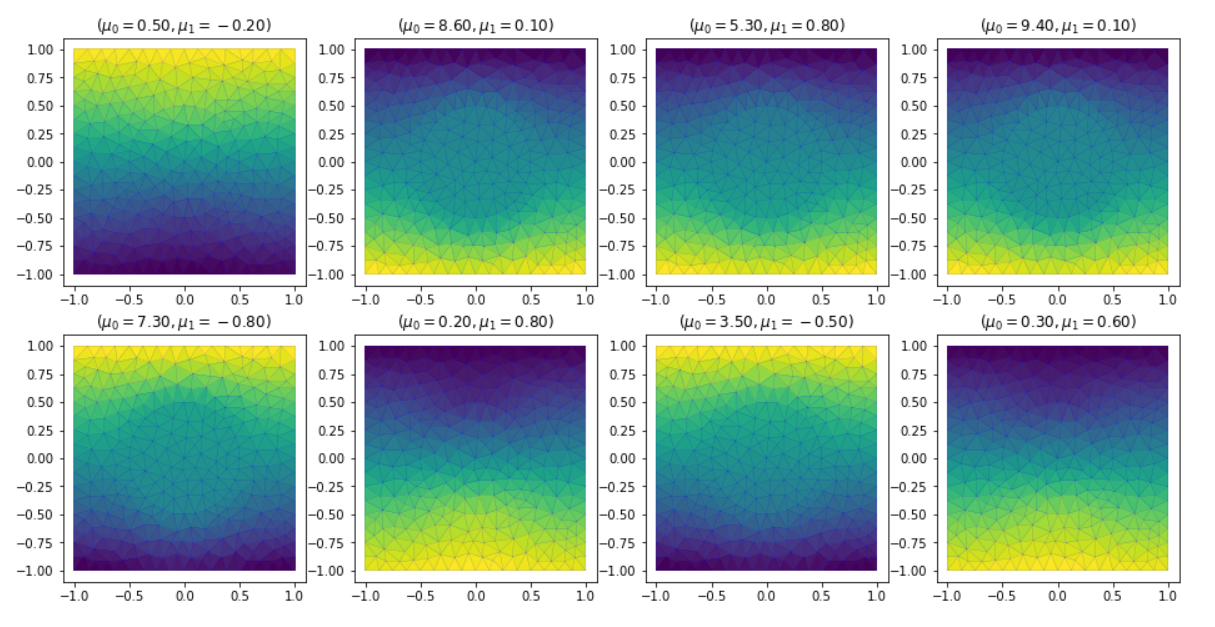
\includegraphics[width=\textwidth]{../images/snapshots}
	
	
\end{frame}

\begin{frame}{EZyRB}
	\Large{\highlightB{Singular values}}
	\normalsize
	
	\centering
	\scalebox{0.75}{
		% This file was created by matlab2tikz.
%
%The latest updates can be retrieved from
%  http://www.mathworks.com/matlabcentral/fileexchange/22022-matlab2tikz-matlab2tikz
%where you can also make suggestions and rate matlab2tikz.
%
\definecolor{mycolor1}{rgb}{0.00000,0.44700,0.74100}%
\definecolor{mycolor2}{rgb}{0.85000,0.32500,0.09800}%
\definecolor{mycolor3}{rgb}{0.92900,0.69400,0.12500}%
%
\begin{tikzpicture}

\begin{axis}[%
width=4.521in,
height=3.566in,
at={(0.758in,0.481in)},
scale only axis,
xmin=0.25,
xmax=8.25,
xlabel style={font=\color{white!15!black}},
xlabel={POD modes},
ymin=0,
ymax=950,
ylabel style={font=\color{white!15!black}},
ylabel={},
axis background/.style={fill=white},
axis x line*=bottom,
axis y line*=left,
legend style={at={(0.97,0.97)}, anchor=north east, legend cell align=left, align=left, draw=white!15!black}
]

\addplot [color=mycolor1, mark=+, mark options={solid, mycolor1, scale=2}]
table[row sep=crcr]{%
	1	874.5893 \\
	2	58.1832  \\
	3	48.2328  \\
	4	45.9105  \\
	5	35.5212  \\
	6	23.8663  \\
	7	20.6150  \\
	8	15.4926  \\
};
%\addlegendentry{Eigen values}

\end{axis}
\end{tikzpicture}%
	}
	
\end{frame}


\begin{frame}{EZyRB}
	\Large{\highlightB{Conclusion}}
	\normalsize

	\begin{itemize}
		\item We presented two algorithms to compute the POD in parallel
		\item EVP perfomes better than SVD due to its limited number of operations
		\item Distributing the snapshot matrix is a bottle neck
		\item We presented hybrid parallel strategy for the POD
	\end{itemize}	

	\vspace{5mm}

	\Large{\highlightB{Outlook}}
	\normalsize
	
	\begin{itemize}
		\item The performance of the computation of the \highlight{correlation matrix} could be improved by using graphics processing units (\highlight{GPU}).
		\
	\end{itemize}
\end{frame}

\begin{frame}{EZyRB}
	\Large{\highlightB{PODmodes}}
	\normalsize
	
	
	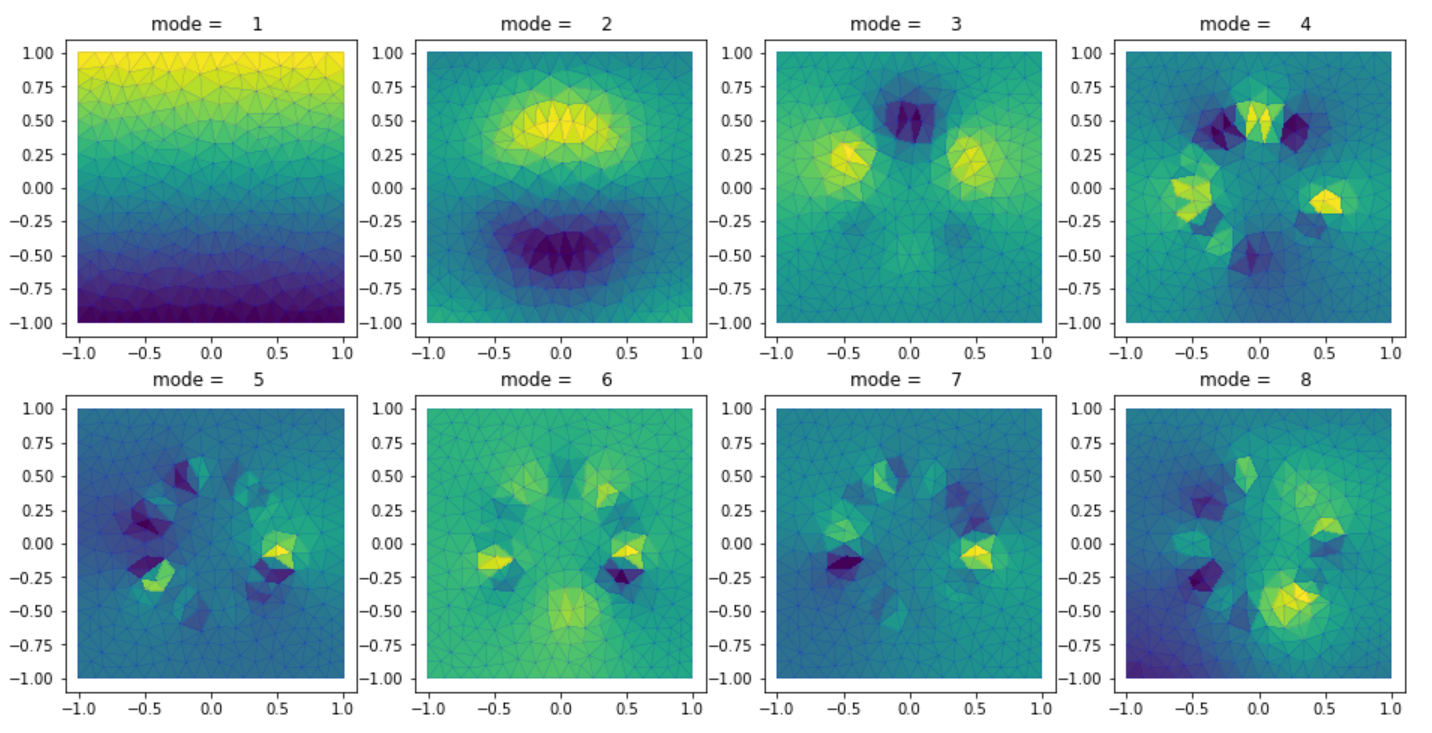
\includegraphics[width=\textwidth]{../images/PODmodes}
	
\end{frame}







\end{document}